\documentclass[12pt,numbers=noenddot,parskip,bibliography=totocnumbered,listof=totocnumbered,draft]{scrreprt}
\usepackage[paper=a4paper,left=30mm,right=25mm,top=30mm,bottom=30mm]{geometry}
\usepackage[utf8]{inputenc}
\usepackage[hyphens]{url}
\usepackage[english]{babel}
\usepackage{lmodern}
\usepackage[sort&compress]{natbib}
\usepackage{graphicx} 
\usepackage{subcaption}
\usepackage{rotating}
\usepackage{pgfplots}
\usepackage{transparent}
\usepackage{multirow}
\usepackage{tikz}
\usepackage{scrextend}
\usepackage{tabularx}
\usepackage[final]{listings}
\usepackage{relsize}
\usepackage{pifont}
\usepackage{enumitem}
\usepackage{setspace}
\usepackage{mathtools}
\usepackage{amsmath}
\usepackage[automark]{scrlayer-scrpage}

% Stil der Seiten
\pagestyle{scrheadings}
\clearscrheadfoot

%Abstand der Fussnoten
\deffootnote{1em}{1em}{\textsuperscript{\thefootnotemark\ }}

%Abstände für Absatzbereiche
\RedeclareSectionCommands[
    beforeskip=-3.25ex plus -1ex minus -0.2ex,
    afterskip=1sp,
    indent=0pt
  ]{paragraph,subparagraph}

%Zeilenabstand
\onehalfspacing

%Regeln, bis zu welcher Tiefe Überschriften angezeigt werden sollen (Anzeige der Überschriften im Verzeichnis / Anzeige der Nummerierung)
\setcounter{tocdepth}{3}
\setcounter{secnumdepth}{3}

%Kopfzeile (Kapitel / Standard)
\ohead{\transparent{0.5}\headmark\transparent{0.5}\transparent{1}}

%Fußzeile (Kapitel / Standard)
\ofoot[\rlap{\hspace{.5cm}\rule[-0.7ex]{.8pt}{\baselineskip}\hspace{.5cm}\pagemark}]{\rlap{\hspace{.5cm}\rule[-0.7ex]{.8pt}{\baselineskip}\hspace{.5cm}\pagemark}}

%Kapitel in Kopfzeile ohne Zahl
\renewcommand*{\chaptermarkformat}{}

%Schriftarten
\addtokomafont{pagenumber}{\sffamily \upshape}
\addtokomafont{pageheadfoot}{\sffamily \upshape}\usepackage[defaultfam,light,tabular,lining]{montserrat}
\usepackage[T1]{fontenc}
\renewcommand*\oldstylenums[1]{{\fontfamily{Montserrat-TOsF}\selectfont #1}}

% Auflistungen
\DeclareTOCStyleEntry[dynnumwidth]{tocline}{figure}
\newcommand*{\adddot}[1]{#1\unskip.\hfil}
\setkomafont{labelinglabel}{\textit}
\graphicspath{ {img/} }
\setlist[itemize]{wide, itemsep=0pt, parsep=\medskipamount}
\addtokomafont{caption}{\small}
\addtokomafont{captionlabel}{\small}

% pgf-Settings
\usetikzlibrary{matrix,positioning,arrows,automata,fit}
\pgfplotsset{compat=newest}
\pgfplotstableset{col sep=semicolon}
\pgfdeclarelayer{background}
\pgfsetlayers{background,main}

% Code
\lstdefinelanguage{cypher}{
  keywords={CALL, CREATE, LENGTH, CONSTRAINT, ON, INDEX, UNIQUE, DETACH, DELETE, DROP, FOREACH, LIMIT, LOAD, CSV, MATCH, MERGE, OPTIONAL, ORDER, BY, REMOVE, RETURN, SET, SKIP, START, UNION, ALL, WING, USING, JOIN, PERIODIC, COMMIT, SCAN, WITH, WHERE, AS, AND, DISTINCT, CONTAINS, ENDS, IN, IS, NOT, NULL, OR, XOR, CASE, COUNT, COLLECT, DESC, TOFLOAT},
  morecomment=[l]{//},
  morestring=[b]',
  morestring=[b]",
  keywordstyle=\bfseries,
  identifierstyle=\ttfamily,
  commentstyle=\ttfamily,
  stringstyle=\ttfamily,
  sensitive=true
}

\lstset{
   language=cypher,
   extendedchars=true,
   basicstyle=\footnotesize\ttfamily,
   numbers=none,
   tabsize=2,
   breaklines=true
}

\begin{document}
	
% TItelseite
\begin{titlepage}
\null
\vfill
% The Collective Guide: A machine for collective recommendations and its desire for disclosure
% Honestly transforms experiences in a collective into public recommendations
% The Honest Machine: Transforms experiences in a collective into honest recommendations
% The bold attempt of transforming experiences in a collective into  recommendations
% The Honest Machine: The attempt of converting experiences in a collective into honest recommendations

% Felix: Sollte beinhalten...
% Recommendation
% Virtuell vernetzt bzw. wohnt im Netz
% Keine Negation
% Freizeitgestaltung verbessern

\Huge\textbf{Free your free time}
\bigskip\\
\LARGE{ Assessment of a machine to increase spare time spent collectively}
\medskip\\
\Large{Jan-Hendrik Wolf}
\vfill
\vfill
\vfill
\small{Thesis submitted to the University Bremen in partial fulfillment of the requirements for a M.Sc. degree in Digital Media\\
Bremen, 30. Juli 2017}
\end{titlepage}

% Anfang des Bodies
\pagenumbering{roman}

%Inhaltsverzeichnis
\tableofcontents

\chapter*{Abstract}

\chapter{Introduction}
\pagenumbering{arabic}
Gone are the days of leisure and self-determined free time. Gone are the days of accepting boredom and time of waiting. The influence of media changed the way we organize our free time.  

Social networks like Facebook or search engines like Google opened up enough opportunities to choose from and made it unreasonable to feel boredom and vacancy, which was an acceptable part of our free time thirty years ago. Not staying in touch over a certain timeframe is not taken for granted anymore due to the growing number of channels in communication. We stress ourselves, trying to fill any possible gap in our free time. Any intervening period during a bus ride, in the waiting room or alone at home is filled with a constantly growing abundance of minor activities. Maintain your friendships, social web profiles and all manner of incoming information. The digitalization \footnote{With digitalization I refer to the integration of digital technologies into our everyday life by the digitization of everything that can be digitized \citep{digitalization}.} made all this possible and the smartphone is the most popular toolbox to pursue these habits. %quelle (are they already habits?)

This development is continued by examples like shopping malls become larger, the number of sports grows and even ordinary commercial products are sold as a new experience. This confusing number of opportunities make us feel afraid to miss a thing. We are constantly trying to transform interims into productive free time, anyhow refuse ourselves to the unexpected. According to a series of studies \citep[p. 14]{freizeitmonitor2016}, we are constantly increase our personal stress level this way. The apparent impression is built up that we are running out of time. 

This phenomenon has impact on the way we spend our free time. The winning activities for the last five years had been activities you are doing alone, whereas social activities had been the most notably losers. It seems evident that it takes more time to meet and spend time with each other personally, than staying in contact via messengers and social media. However, why do we not use the advantages of computer technology in a way that motivates people to preferably spend their free time in a context of social activities again? Is it possible that an application, the embodiment of the digitalization, can invert the trend towards a free time with social activities in focus? % <-- question / discuss

The thesis will call attention to the constant change of one's free time under decades of digital influence. It will investigate to what extend the ubiquitous accessibility of everyones attention certainly played its part to this development and proposes a possible solution to invert the trend. A puristic application that does not focus on chat components, self-portraits and its time-consuming relatives. The aim is to conceptualize and implement an application that helps to organize one's free time with a small timestamp online and its constant motivation, in contrary to existing solutions like Facebook, to make people meet each other in person again rather than digitally. The thesis will end with an evaluation of the application to validate whether it is a rather drastic and humorously ironic idea to come up with another digital application or a step forward to one's organization free time with more social activities.

\chapter{The Evolution Of Free Time}

The following chapter gives a general definition of free time that is used in the context of this thesis. The second section provides a historical overview of the development of free time and summarizes key changes towards a society of time pressures. In order to compare the machine to alternatives, other contemporary organization tools are discussed at the end of this chapter.

\section{Definition}

There is an ongoing progress of defining free time in leisure studies. Several definitions of free time and leisure time have been constituted in multiple ways. German leisure studies distinguish between positive and negative definitions of leisure. 

Originating in the protestant work ethic \citep[p.27]{weber2006} and industrialization, negative definitions of leisure describe the time off from non-eligible activities, including employment, transit time, hygiene and eating \citep[p.137]{prahl2002}. Unfortunately these definitions partially exclude individuals, who are unemployed, elderly or teenagers. \citeauthor{scheuch1972} tries to overcome this major weakness of negative definitions and suggests to set the type of activity in relation to the functional role of the individual in society. Leisure time is not meant to be a quantitative time unit anymore, but is rather defined as a phenomenon of its own \citep[p.31]{scheuch1972}. With \citeauthor{scheuch1972} the development of new definitions of leisure started.

Positive definitions of leisure focus on the fact, that an activity ``has been chosen primarily for its own sake, for the experience itself'' \citep[p.15]{freysinger2000}. Quality becomes the predominant feature of leisure\footnote{In most cases, it is easy to determine, whether someone enjoys an activity and feels satisfied. Consequently positive definitions are a good way to distinguish between leisure and non-leisure time. But does an individual spend leisure time by doing sports in the gym to loose weight? Does a pop band, who plays for a hobby, have leisure time at a party when asked to play, although they rather would like to enjoy the party without performing? Sometimes it is not possible to distinguish, whether someone is spending leisure or non-leisure time. Only the persons themselves can tell.} and is no longer soley bound to time. Positive definitions of leisure are the most common way of defining leisure internationally.

In international leisure studies the definitions of free time are comparable with negative definitions of leisure mentioned above. The American sociologist \citeauthor{stebbins2007} describes free time as the ``time away from unpleasant obligation'' \cite[p.4]{stebbins2007}, as a quasi subtraction of the unpleasant from one's totally available time. \citeauthor{stebbins2007} definition shows little variation to negative definitions of leisure. In accordance with positive definitions of leisure \citeauthor{stebbins2007} defines leisure as an ``uncoerced  activity engaged in during free time, which people want to do and, in either a satisfying or a fulfilling way (or both), use their abilities and resources to succeed at this''. 

There are numerous definitions of free time and leisure and the entire field is complex. In this thesis My discussion in this thesis will use the definitions constituted by \citeauthor{stebbins2007} as his statements are well applicable to positive and negative definitions of leisure. In summary, \textit{free time} in this thesis is meant to be the time away from eligible activities, whereas \textit{leisure time} corresponds to executing uncoerced activities leading to fulfillment and satisfaction.
 
\section{Historical Development}

The emergence of free time is a result of a large set of historical developments. An awareness of free time cannot be developed without the awareness of time. Long before humans used tools to map time onto a scale, time was mostly perceived in a cyclic manner, regarded as a succession of recurring phases. The alteration of day and night, the intake of food, recurring rituals or seasonal phenomena are examples of the very beginning of an awareness of time. The mapping of time onto a linear scale, which allows to define a specific point in time as well as to measure the duration of activities, was introduced by the ancient Egyptians with the sothic cycle and the first sundials. \citep[p.25-27]{whitrow1989} The precision was coarse and varied in different regions of the world until centuries later mechanical clocks raised the precision to a practical level \citep[p.103]{whitrow1989}. However, it was primarily the reformation and the accompanying protestant work ethic that paved the way for an economization of time as part of European capitalism \citep[p.22]{weber2006}.

With the industrial revolution, factory workers had to align their division of time to the rhythm of machines. They lost the freedom of allocating autonomously their working-hours. \citep[p.160]{whitrow1989}. With industrialization a clear distinction of free and working time became possible. Basically, time is bound equally to each one of us and cannot run short. Money is the collectible counterpart and can be transferred to other individuals independently. As loan was now solely coupled to working hours, the evaluation of time with money transformed time into a scarce resource that each individual was able to sell to employers \citep[p.54]{marx1867}. 

The industrial revolution did rise the number of working hours to a maximum \citep[p.98]{prahl2002}. It also initiated a large set of ongoing processes to streamline and densify time in line with the maxim ``time is money'' - the famous statement by one of the founding fathers of the United States of America, Benjamin Franklin \citep[p.22]{weber2006}. The invention of the railroad introduced the standard time as it became necessary to have a unified time across cities. The telegraph and the undersea cable boosted the communication and shortened the physical distance between people. Shortly after, mass production of pocket watches started. Watches became ubiquitous and began to dominate everybody's life - Lewis Mumford said, ``the clock, not the steam-engine, is the key-machine of the modern industrial age''. \citep[p.161]{whitrow1989} The densification of time continued with the invention of electricity and the light bulb that leveraged the alteration of day and night. With the spreading of roll film cameras people were able to easily capture and fix every thinkable situation in time. At the beginning of the 20th century, the first mass production of cars (e.g. Ford Model T) and airplanes further decreased the physical distance and increased the traveling speed. \newline
Among the densification until the middle of the 20th century, the number of working hours decreased due to the efforts of the labor movement and social policies. It has since been recognized that the mass production and the resulting high supply of goods cannot persist without a respective demand. Consequently, the amount of free time increased. \cite[p.99-100]{prahl2002} With the advent of additional free time, the demand for a higher quality of free time increased and it's commercialization started.\citep[p.116]{scheuch1972} The growing wealth also increased the number of leisure facillities. Different flows of leisure oportunities greater occupied people's free time along all social classes: The mass media made it possible for workers to listen to operas of the high class. New music and dancing styles were developed. New kinds of art got published and even new life styles had been tried out. Free time gained a new quality. \cite[p.106]{prahl2002}

In the mid 20th century many countries finally had been established the five-day workweek\footnote{In Germany the trade union DGB titled ``Samstags gehört Vati mir'' (german for ``At saturdays dad is mine'').}. In western countries free time gradually transformed into a time of mass consumption. The notion of performance in our working-life had been applied to each individuals free time, competing with consumption, status symbols, travel and leisure performance in general. \citep[p.112]{prahl2002} Additionally, flexible working-hours decreased the ability of individuals to find matching timeframes for social activities with friends and family members. \citep[p.75]{wajcman2014}

In the end of the 20th century, the invention and the ongoing emergence of the world wide web initiated another intensive densification of time. The complexity of information that can be transferred at a time increased spectacuraly \citep[p.45]{wajcman2014}. The best breeding ground for a sheer expansion of the globalization. The distances of global trade had been almost made meaningless as people were able to send different kinds of information in real time \citep[p.17]{wajcman2014}. The competition intensified and time is even more money and a timeframe of an individual becomes more precious. Besides the rise of globalization, the information age also changed the way people communicate personally. The communcation via the world wide web became ubiquitos. The technology makes it possible to correspond to more people at a time, than ever before. In addition, messengers and mails allow to schedule replies whenever possible without consuming time in meetings and goodbyes. The society transformed itself into an ``always on'' culture that puts the focus on being always available. No one is forced to do so, but social pressure encourages and spreads it. Responding late is not welcome in a ``norm of responsiveness` \citep[p.96]{wajcman2014}. A time for a break is rare. The type of communication of each person does not even stop when it is of no importance. Privacy and the quality of communication decreases in favor of speed.

An ever-accelerating communication is the result of technological progress that is likely measured by time-saving benchmarks. Increasing the speed in transporation and communication technology is certainly desireable. Faster means of transportation\footnote{The Hyperloop One will need less than a hour to transport people from Melbournce to Sydney. The company says it is not ``seeling transportation, [it is] selling time''. \cite{hyperloop2017}} increases the comfort in trading and travelling. Unfortunately, a multi-option society with intense pressure on performance makes people feel a necessity to keep up. People fall into a pressure of realization and invest their time saved personally in additional activities and information exchange to increase the activities and correspondences per day instead of making room for leisure \citep[p.27-30]{gross1994}.

\section{Present Development}
The historical development towards an always-on society strongly influences today's lifestyle. The following section mentions several statistics and behaviors of present leisure time in the 2020s.

\begin{figure}
\centering
\begin{tikzpicture}
\begin{axis}[xbar,
    width=0.66\textwidth,
    tickwidth = 0pt,
    xtick=\empty,
    enlarge x limits=0.25,
    y axis line style = { opacity = 0 },
    y=0.75cm,
    ytick = data,
    yticklabels from table={plotdata/topactivities.csv}{Activity},
    yticklabel style={align=right,anchor=east},
    xlabel={Ratio of people executed the activity by 2016 [\%]},
    xlabel style={align=right},
    nodes near coords={\pgfmathprintnumber[fixed zerofill,precision=0]{\pgfplotspointmeta}$\%$}
]  
\addplot [fill=white] table [y expr=\coordindex, x=Percentage]{plotdata/topactivities.csv};
\end{axis}
\end{tikzpicture}
\caption[Most mentioned activities]{The study conducted by \citep{freizeitmonitor2016} surveyed 3000 people over the age of 14 years in face-to-face interviews. Participants were asked to name their leisure activities of the past week. The chart shows the most mentioned activities.}
\label{topleisureactivities}
\end{figure}

The broad range of leisure opportunities and an ongoing densification of time influences the way we choose activities during free time. According to \citeauthor{schulze2005} there are six forms of existence\footnote{\citeauthor{schulze2005} differentiates between six modes of existence between situation and subject. The situation can \textit{constrain} one's actions, for example by law regulations, liquidity or the time of day. Alternatively, a situation can \textit{encourage} and \textit{trigger} actions of a subject. The subject may use \textit{symbolization} to let other subjects interpret it, like showing material wealth by wearing expensive clothes. The subject can change the situation by \textit{choosing} from a given set of possibilities or \textit{influencing} it by changing the set of possibilities manually. \citep[p. 198-206]{schulze2005}}. It seems like today's time pressure lets people rather stay in the form of existence to ``choose'' existing activities instead of ``influence'' things by their own. In other words, instead of being a musician yourself, you go to a musical event and listen to professional artists. This allows time savings and professional music enjoyment at the same time. In a networked world, things are easily accessible from everywhere and people tend to develop higher expectations on leisure activities. This begins primarily for children as soon as they have access to interactive media, which often provide little space for one's own personal level of imagination. Compare a computer game with a book or a construction kit - a computer game with highend graphics can come with complete visual and audiovisual information, whereas the book and the construction kit are incomplete enough to make room for fantasy. Ever-faster communication and global competition support and promote this form of existence. Meanwhile, a large number of leisure activities are available to meet a strong demand. The market has become highly complex for many people. Although recommendations from friends or acquaintances for leisure activities are valuable and trustworthy, it is not uncommon to consult other information sources via multiple channels. According to a conducted study by \citeauthor{freizeitmonitor2016}, six of the top ten most done leisure activities are media-related as shown in figure \ref{topleisureactivities}. This affinity to media and the large number of leisure activities explains the existence of various magazines, radio programs, TV formats and websites\footnote{An incomplete list of examples in these channels: ``Kultur heute'' (program by german radio station ``Deutschlandfunk), ``Das ist los im Norden'' (program by north german radio station ``ffn''), ``MIX'' (german magazine and website - operates in Bremen, Bremerhaven and the surrounding area), ``www.wasgehtheuteab.de'' (german website - operates in Germany), ``eventful.com'' (american website - operates worldwide), ``eventim.de'' (german website - operates worldwide), ``eventbrite.de'' (american website - operates worldwide), ``'ttt - titel thesen temperamente'' (program by german television channel ``ARD'').}. Apart from the strong media consumption, \citeauthor{freizeitmonitor2016} extracts two additional major groups. The following main groups were identified:

\begin{labeling}{regeneration}
\item[media use] This involves the use of classic and new media formats. Especially young people use the internet as a tool to coordinate activities or maintain social contacts.
\item[regeneration] The traditional regeneration after work is still an important part of modern leisure activities.
\item[socialize] The purpose of this major group is to spend leisure time together with family, friends and acquaintances.
\end{labeling}

The same study reveals that 98\% of young adults used the Internet in the last week, which makes the internet the most popular leisure activity in this age group \cite{freizeitmonitor2016}. Thus, the internet is likely to be the most popular source for young adults today. 91\% of young adults said that they had been active in social media in the last week \cite{freizeitmonitor2016}. Facebook is the largest social network and explains on one of its marketing sites that 440 million people use the event features alone on Facebook - 35 million of them daily \citep{facebook2017}. In the year of 2015, around 47 million events were created on Facebook \citep{facebook2017}. A social network can use its strengths in this field to give individualized information to people. The network either returns a list of potential attendees or recommends events of interest, like those organized by friends. In a digitized world, automated recommendations coexist and possibly compete in various fields with those given by acquaintances and friends.

The disadvantage of communicating via social networks, instant messaging services and similar methods is that they make it unnecessary to meet in person anymore. This extensive use of these communication technologies in conjunction with the perceived scarcity of time have an impact on the way we spend our free time. As shown in figure \ref{topfivechangingleisureactivities}, the 5-year comparison shows that primarily common activities show the highest drop rate, whereas solitary activities show the highest growth in this trend. This is worrying, but not an unusual development. The personal presence of people is becoming increasingly unimportant with social networks and comparable technologies, as they seek to establish themselves as a medium in between. Interpersonal relationships also suffer from the already mentioned rationalization of time in which ever arising time gaps are being filled. Social media become the passive communication channel through which people make their experiences available to the public. This way, leisure time has become part of one's self-promotion and is therefore increasingly subject to a performance principle, just like employment does.

\begin{figure}
\begin{tikzpicture}
\begin{axis}[xbar, 
    enlarge x limits=0.25,
    xtick=\empty,
    width=0.66\textwidth,
    tickwidth = 0pt,
    y=0.75cm,
    y axis line style = { opacity = 0 },
    ytick = data,
    yticklabels from table={plotdata/trendofactivities.csv}{Activity},
    yticklabel style={align=right,anchor=east},
    xlabel={Ratio of people executed the activity by 2016 compared to 2011 [\%]},
    xlabel style={align=right},
    nodes near coords={\pgfmathprintnumber[fixed zerofill,precision=0]{\pgfplotspointmeta}$\%$}
]
\addplot [fill=white] table [y=Position, x=Percentage]{plotdata/trendofactivities.csv};
\end{axis}
\end{tikzpicture}
\caption[Trending and abonding leisure activites]{Top-five trending and abandoning leisure activities done at least once a week in a 5-year comparison by those polled. \citep{freizeitmonitor2016}}
\label{topfivechangingleisureactivities}
\end{figure}

Social networks provide a good overview on the large number of leisure activities. However, this ability is just a small subset in the functional scope of social networks. Sadly, the previously presented statistics seem to demonstrate that it does not encourage people to do activities collaboratively. The incentives to meet in person may be insufficient in social networks. By taking certain precautions and by focusing on collaborative activities, it may be possible to tackle this development.

\chapter{The Machine}
This chapter presents the conception and implementation of a machine that has the aspiration to provide people an organizational assistance to plan their free time with fellow people. An imaginable scenario is the desire of a person to be active in sports and to practise a sport that is unfortunately less popular. The person resides in a city that does not have a club offering the sport. This is why the person would like to find like-minded people to do sports together. In another case, a group of people would like to attend an event with standard group sizes. To save money, the group is looking for another person to complete the next greater group size. In the last scenario, somebody would like to take a cultural tour around the city and is looking for nearby events, which are not necessarily listed in the event calendar. All scenarios require a dedicated point to call for advice. Existing unidirectional tools, such as the event calendar in magazines, do not provide the necessary level of interactivity to locate interested people. In addition, bi-directional tools, such as social networks, prioritise other issues and do not focus on an effective planning of events. This leads to a higher potential for distraction and therefore increases the chance to spend more time online as needed to organize offline time.

As part of the conception, precaution is taken and reviewed to respect the mentioned developments in free time. To complete the description of the machine, important aspects of the later implementation are explained in detail, in which the concept constitutes its foundation.
% minimal eingreifend und einschneidend, maximal die Selbständigkeit fördernd.Jeder verbringt und plant seine freizeit unterschiedlich. Eine Frage der Qualität. Ein Schichtarbeiter wird seine Freizeit sicherlich anders gestalten, als ein Beamter, der täglich zur gleichen Zeit nach Hause kommt.

\section{Concept}
Although smartphone applications are the epitome of digitalization and thus make a decisive contribution to our feeling of time pressure, the machine should be based on a smartphone application. This is intended to investigate whether it is the technology or the design of such applications that causes us to be short of time. The following concept aims to shorten the time spent organizing activities in favor of time spent qualitatively. In this sense, the individual also spends more leisure time. 

A clear distinction between leisure time and free time can be problematical, once applied for the general public. While many people consider shopping to be a necessary part of their daily routine, shopping on vacation can be fun as a stopover on a day trip. Thus, the respective boundaries between leisure time and free time are defined by subjective aspects, for example  Consequently, the boundaries are fuzzy in an objective context and it is difficult to find suitable constraints. For this reason, maximizing leisure time cannot be considered as the primary goal. Instead, the machine is intended to expand leisure time only and thereby optimize free time. The following sections explain how the application is supposed to decrease online time in favor of offline time as well as the basic idea of the application.

\subsection{Guideline}
This section lists five statements that aim to decrease the amount of online time in favor of offline time. Every statement is introduced with an underlying explanation.

\paragraph{Statement 1: Stop thriving self-promotion online}
The first statement to increase leisure time is the intention of a strong restriction on an individual self-promotion. As an essential part of the comprehensible intrinsic need to be liked by others, self-promotion influences the way we clothe and express ourselves. However, it can be overly optimized on social media as the individual is able to decide what to share with the public. The individual can build up their own personalities, manipulate their outer appearance and the surrounding environment. I think it is reasonable to say that individuals economize their self-promotion for likes and shares on social media. This ever-improved false picture let individuals become more and more subject to a greater social pressure to compete with the apparent norm of a gradually optimized presentation of everybody's personality \citep{jay2012}. Thus, the individual spends more time on social media to maintain their profiles and to keep part of the discussion. Studies show that there is a correlation between somebodies relative happiness and the hours spend as well as the number of years registered on Facebook \citep[p.119]{chou2012}.\newline
In order to decrease the time spent on such activities, the machine has a reduced number of possible spaces thriving self-promotion. Only a profile photo and a short description of the person shall be allowed. This way, new members have the ability to introduce themselves to the community and everybody can get an idea of each other. However, there will be no further interactive elements to shape one's self-promotion. This design prevents possible competitions along members in the context of self-promotion and shall free up space in everybody's free time.

\paragraph{Statement 2: No social feeds or unrelated features}
The second statement calls for an avoidance of secondary features that are not essential for organizing activities. Secondary features may include the display of an advertisement, news and any kind of social feeds. A social feed allows individuals to upload videos, status updates or photos. As the essential part of their business models, most social networks engage community members to contribute or interact with the social feed. This way, the social feed is an awarding advertising space. A higher engagement and retention time means more ad-placements and a higher profit. Consequently, social media applications like Facebook and Twitter do not reward anybody to meet in person. On the contrary, the more time individuals spend on their platform, the greater is the probability to receive more likes and comments. Most of the people may not have won much in the end. Instead of being active by themselves, they consume the content of the social feeds. In addition, meeting in person would have the advantage of a more conscious communication as facial gestures are an essential part of it  \citep{vanderkam2017}. That is the reason why job interviews and presentations are most likely done in-person \citep{vanderkam2017}. In addition, studies show that in comparison to textual conversations, in-person meetings let communication partners feel more satisfied and increase the level of mutual attention \citep{vanderkam2017}. \newline
In the interest of refocusing to in-person meetings, the machine does not mislead individuals to spend time unnecessarily for other purposes. Thus, the application will not feature a social feed or any kind of advertisement.

\paragraph{Statement 3: Make strong efforts to reduce instant messaging}
The third statement is a limitation of instant messaging. As mentioned in the previous section, in-person meetings have many advantages. In order to keep the motivation at in-person meetings as high as possible, a general chat is not used in the application. Nevertheless, while planning a meeting, it should be possible to communicate with each other online to establish an initial communication.

\paragraph{Statement 4: Make use of machine-generated recommendations}
The fourth statement proposes machine-generated recommendations. As already explained in the previous chapter, there are different sources of recommendations with their own advantages and disadvantages. While friends and acquaintances usually have a more detailed knowledge of a person's personal preferences, machines have the ability to compare a large set of data from large databases to identify analogies. In addition, publishers of magazine recommendations, such as the MIX-Verlag\footnote{The MIX-Verlag is a german publishing house that publishes every month a magazine with event recommendations for Bremen, Bremerhaven and the surrounding area.}, also benefit from a wide spectrum of activities and may even receive insider tips from event hosts and their readers. However, all submitted information is reviewed and finally forwarded to the readers in a filtered format. Consequently, recommendations from editorial sources can be influenced by third parties in a political, financial or local manner. Likewise, recommendations made by acquaintances can also become subject of their respective interests. An acquaintance might decide to withhold a restaurant recommendation from someone as they would like to visit the restaurant undisturbed at the same time.\newline
In contrast, a corresponding algorithm can generate neutral recommendations on the basis of the same parameter types. In addition, community members need to be able to make their own suggestions for activities. As a result, the database becomes more and more extensive and offers an increasing variety of activities and insider tips. Thus, all members in the community define the ground for potential recommendations by interacting with the machine. This is why machine recommendations should also be part of the machine's features.

\paragraph{Statement 5: Keep it simple stupid}
The fifth and last statement sets the requirement of a thought-out human-computer interface that focuses on the most essential features and is designed to keep the time of interaction with the machine as short as necessary. As discussed in the previous chapter, there are many applications for organizing events that have many different features due to their size and thus increase the level of complexity. Although applications with a wide range of features are certainly interesting, these applications have a greater potential for distraction. An application does not have to be very complex to plan events in a comfortable way. \newline
This means that less relevant features, which unnecessarily require one's attention, are excluded from the machine. Instead, it has to be possible to quickly select and manage activities with little effort and within a short time. An explorative page can provide an overview of all local activities in a matter of seconds.

\subsection{Basic Idea}
When people want to spend time together, they are often looking for like-minded people with whom they can carry out a particular activity with pleasure. Because of this reason it is reasonable to give all members the possibility to classify themselves among different groups of interests, so that like-minded people can easily find each other for an activity. In a community of this kind, it should be possible to plan common activities and to add additional people. Before the activities take place, all participants need the opportunity to inform themselves and discuss the detailed procedure. 

On the basis of these principles, one could notice that it is not easy to distinguish between interest groups and activities. Another terminology must be applied to simplify a distinction. Where do we find similar constructs within other areas? In the wildlife, animals group themselves in hordes or packs, depending on their species. While a herd of animals shows strong self-dynamics that may not always meet the individual desires of each animal, there are clear patterns in a pack. Shared characteristics become apparent as soon as one applies the concept of the pack to the group of interests. Hence, a comparison seems to be appropriate. In both concepts each member pursues similar intentions. However, hierarchies and genetic relatedness, as they exist in wildlife, are not required. Thus, I like to use the metaphor of a pack to describe an interest group within the application.

To complete the terminology, a corresponding name for an activity and the application is needed. Every time wolves start hunting, we speak of an expedition. Likewise, such a metaphor applies perfectly to the machine's structure as well. In the context of this application it should be noted that you cannot take hunting literally. The objective is rather the execution of the activity in general by members of any given interest group. This is why an activity will be called an expedition in the context of the application. 

The name of the application should follow the same terminology. To support the acceptance of the application in german-speaking countries and thereby increase the probability of a meaningful evaluation, the german term "Rudel" (pack) can be used. In order to keep the total number of terms small, the group of interests will be entitled after the german translation as well, which is why a group of interest is renamed to "Rudel" (pack). In order to find the application in search results more easily and to differentiate the name of the application from the group of interests, the term can be slightly varied and shortened. In this case, the name "rudl" seems to be a fitting name for this application.

Now that the general idea and its related terminology has been described, the implementation of the application will be explained in the next section.

\section{Implementation}
In this section, various components are presented that are necessary to implement the machine in accordance with the above concept. In this context, a visual language will be presented to encourage a simple interaction between the individual and the machine. Afterwards, the entire structure and layout of the application will be illustrated and how members of the community can organize their leisure activities in line with the concept. At the end of this section, the recommendation algorithm is explained using the corresponding data storage technology.

\subsection{Visual Language} 
The visual language is an underlying rule set for the design of all visual components within the application. A standardized visual language increases the memorability, familiarity and simplifies the overall handling for anyone interacting with the application. In addition, a visual language can create a sense of security. For example, stores of a large coffee house are looking very similar in all parts of the world. The creation of a familiar environment creates a certain feeling of security. As the application is going to operate with personal data, the definition of a visual language therefore offers added benefits.

\begin{figure}
\centering
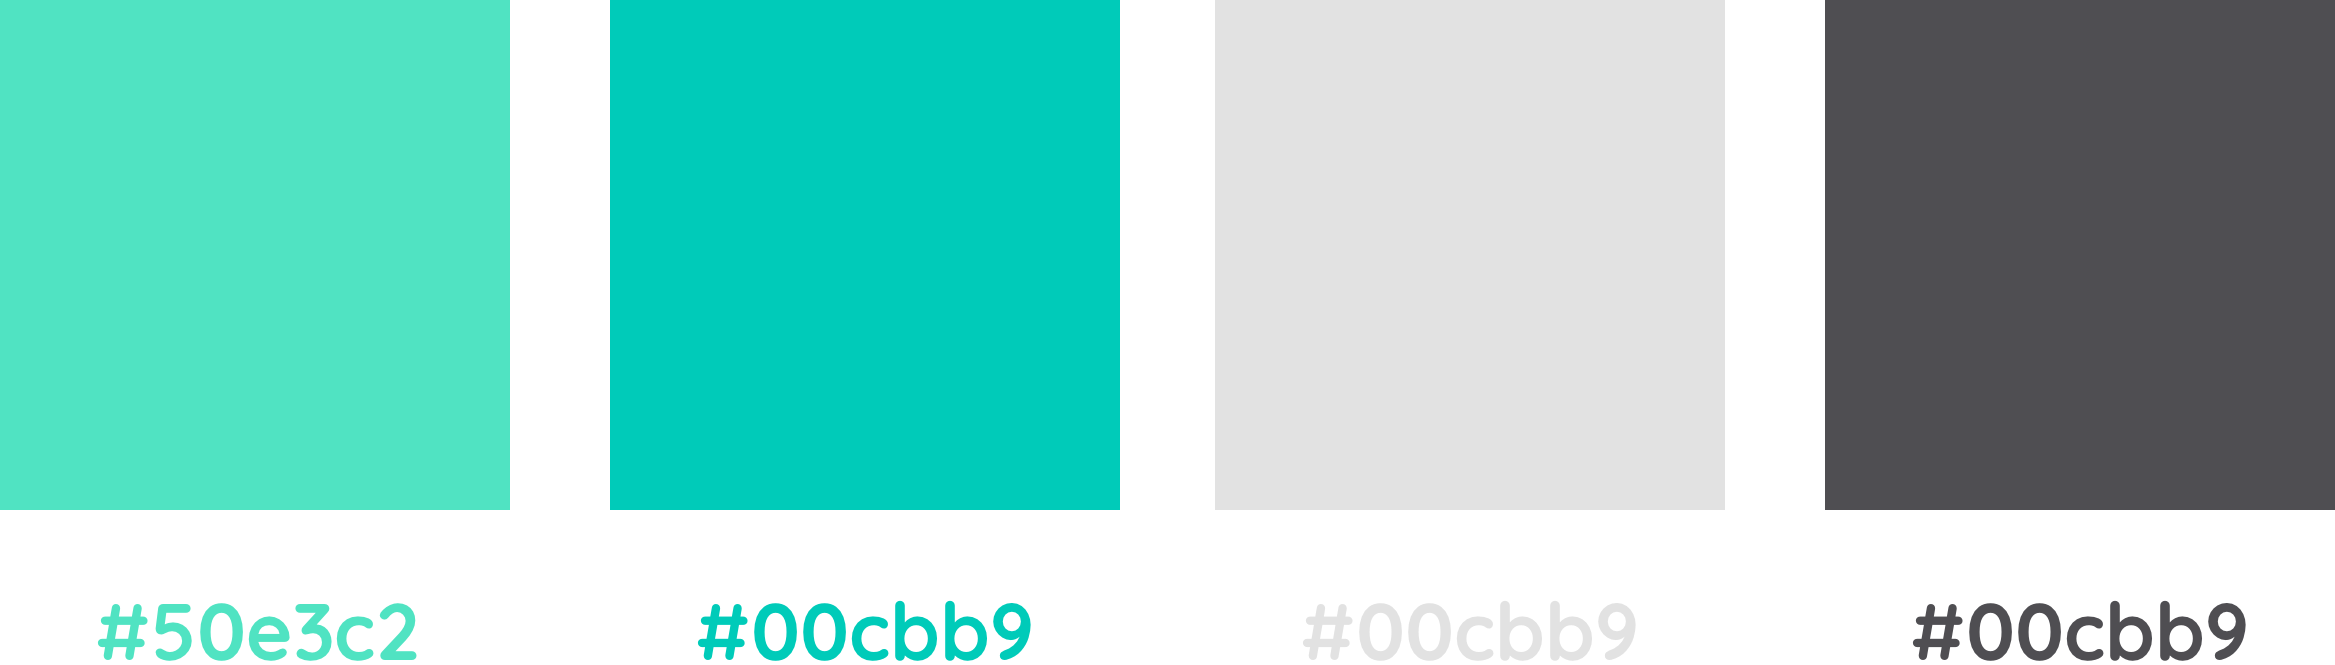
\includegraphics[width=\textwidth]{colors.png}
\caption[Color palette]{Greenish tones define primary and secondary colors and a light color palette.}
\label{colors}
\end{figure}

To ensure that each member associates the metaphor of the pack and the expedition with a positive attitude, it is important to provide a friendly look and feel throughout the entire application. This is why a palette of light colors shall be used. Green nuances influence the primary and secondary colors as shown in figure \ref{colors} to reinforce the metaphor and its relationship to nature. The primary and secondary colors are intended to highlight those components that deserve attention. That includes essential buttons and the logo of the application. In the same manner, the logo of the application draws attention to the concept of packs, expeditions and wolves by illustrating a howling wolf in front of a moon colored in the primary color. In line with the goal of the visual language, simplicity and a high memorability were respected in the design. Figure \ref{icons} shows the final logo with a selection of alternatives and previous iterations.
 
\begin{figure}
\begin{subfigure}[t]{0.45\textwidth}
\centering

\includegraphics[width=\linewidth]{icons.png}
\caption{}
\label{icons}
\end{subfigure}
\hfill
\begin{subfigure}[t]{0.45\textwidth}
\centering

\includegraphics[width=\linewidth]{fonts.png}
\caption{}
\label{fonts}
\end{subfigure}
\caption[Icons and typefaces]{Icons and typefaces as defined by the visual language: Multiple iterations of the logo (\subref{icons}) with different shapes and colors. The non-transparent icon is the final version of the logo. The typeface (\subref{fonts}) consists of two sans serif fonts - Quicksand is used for headings, whereas Lato is used for floating text.}
\end{figure}

Not only the colors and icons contribute to the positive attitude, it can also be influenced by the writing style and typeface. Correspondingly, the typefaces as shown in figure \ref{fonts} are sans serif fonts to ensure the necessary simplicity. Formulated texts shall always make positive statements and do not blame human beings for interaction errors, whenever possible.

As the visual language can ensure a streamlined design of the application, the following sections describe the corresponding features.

\subsection{Organisation of Interest Groups}
\begin{figure}
\begin{subfigure}[t]{0.45\textwidth}
\centering
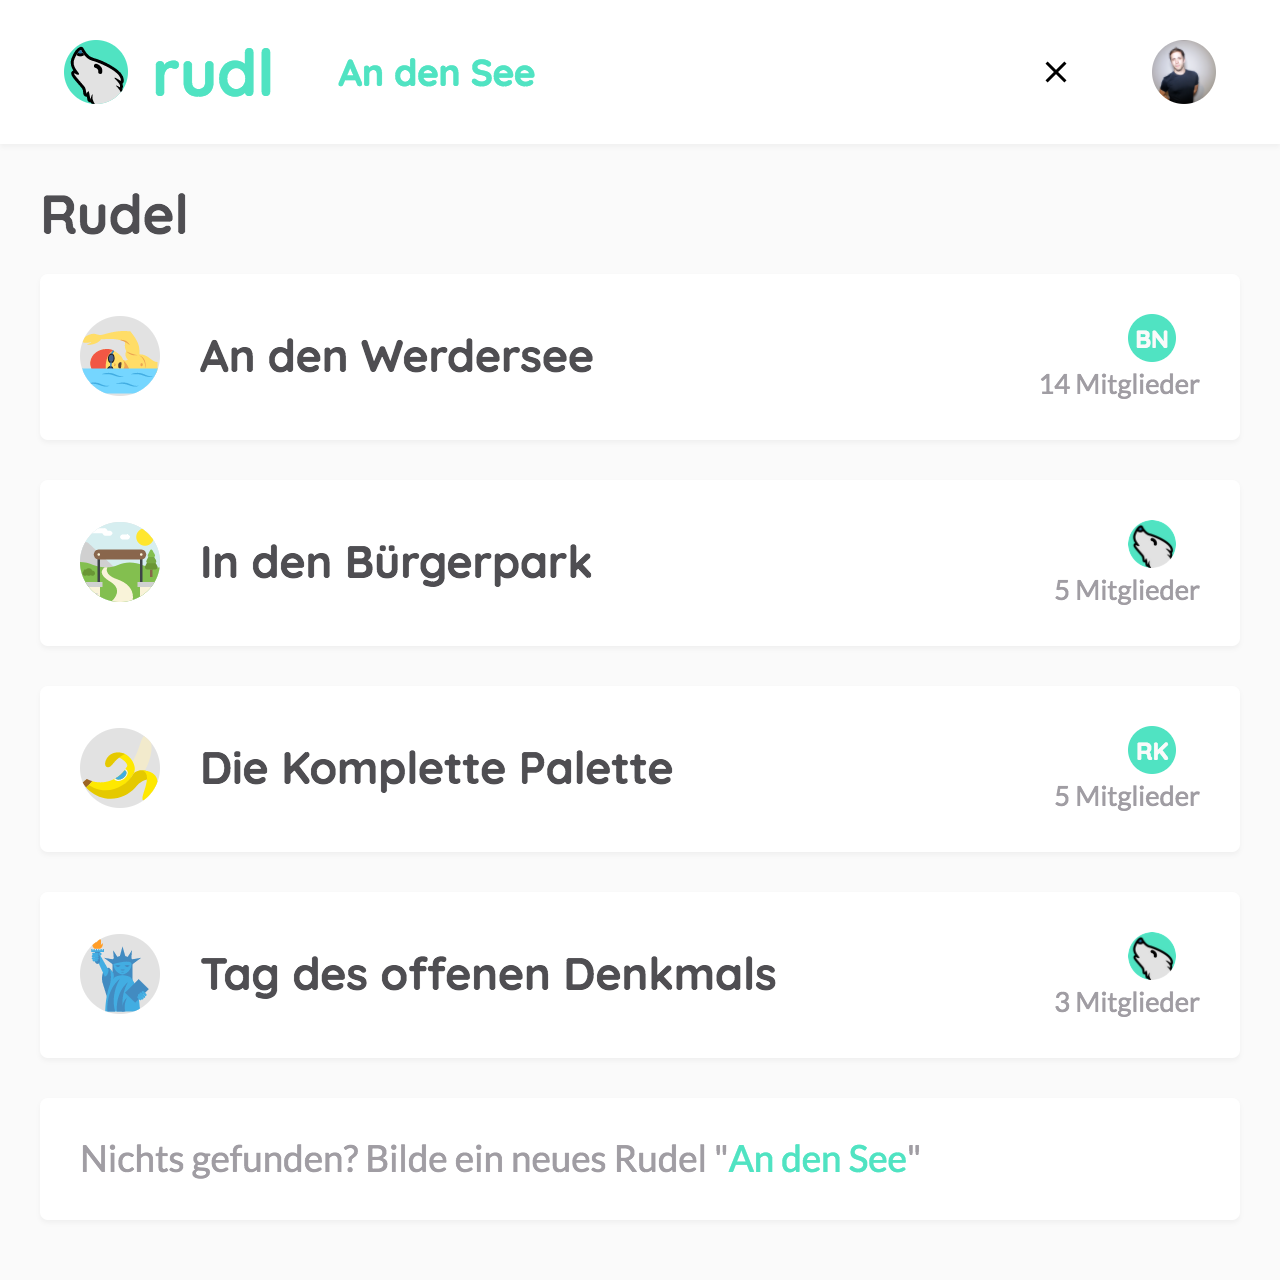
\includegraphics[width=\linewidth]{searchinterestgroup.png}
\caption{}
\label{searchinterestgroup}
\end{subfigure}
\hfill
\begin{subfigure}[t]{0.45\textwidth}
\centering
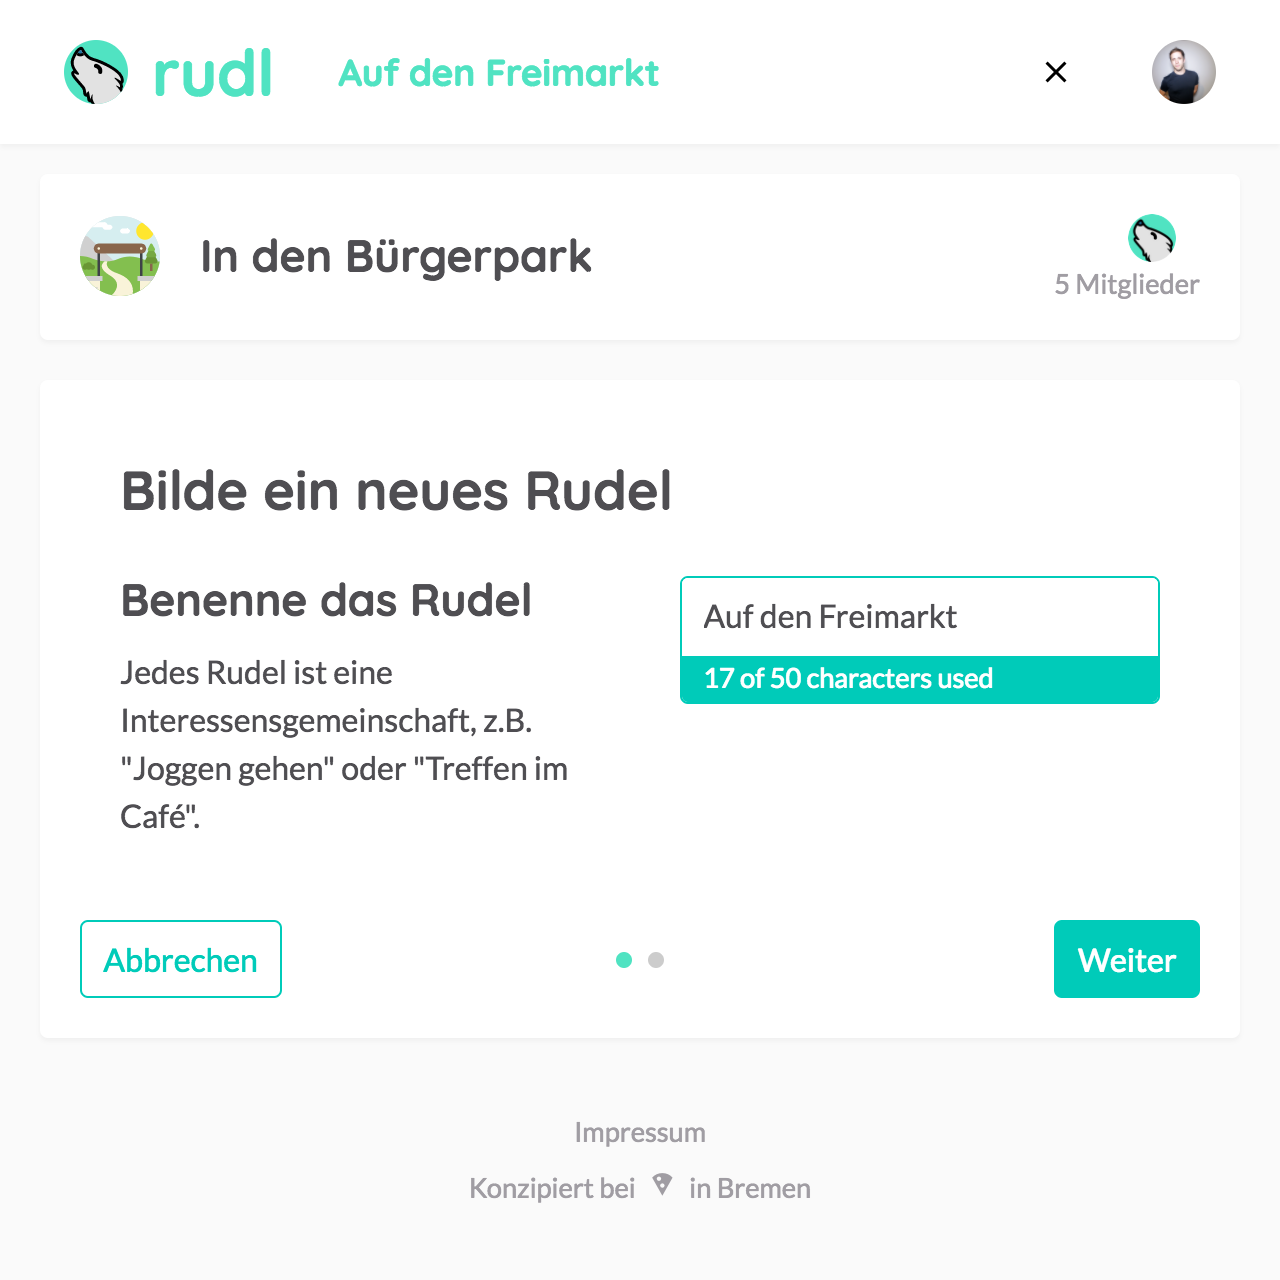
\includegraphics[width=\linewidth]{createinterestgroup0.png}
\caption{}
\label{createinterestgroup0}
\end{subfigure}

\bigskip

\begin{subfigure}[t]{0.45\textwidth}
\centering
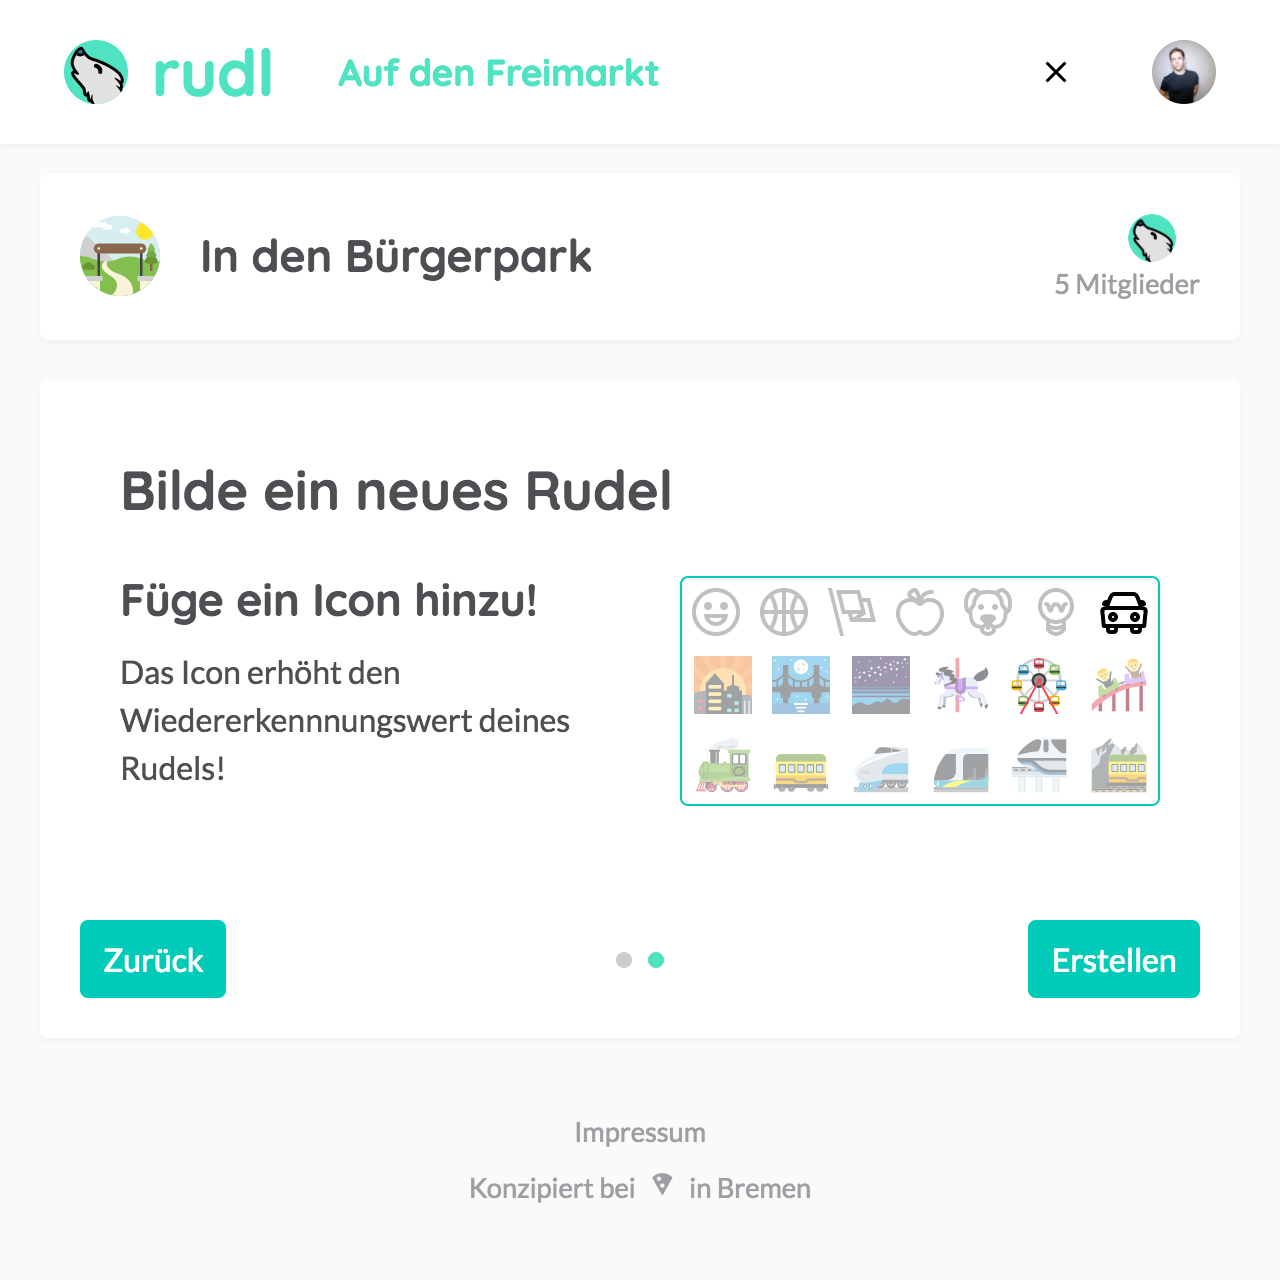
\includegraphics[width=\linewidth]{createinterestgroup1.png}
\caption{}
\label{createinterestgroup1}
\end{subfigure}
\hfill
\begin{subfigure}[t]{0.45\textwidth}
\centering
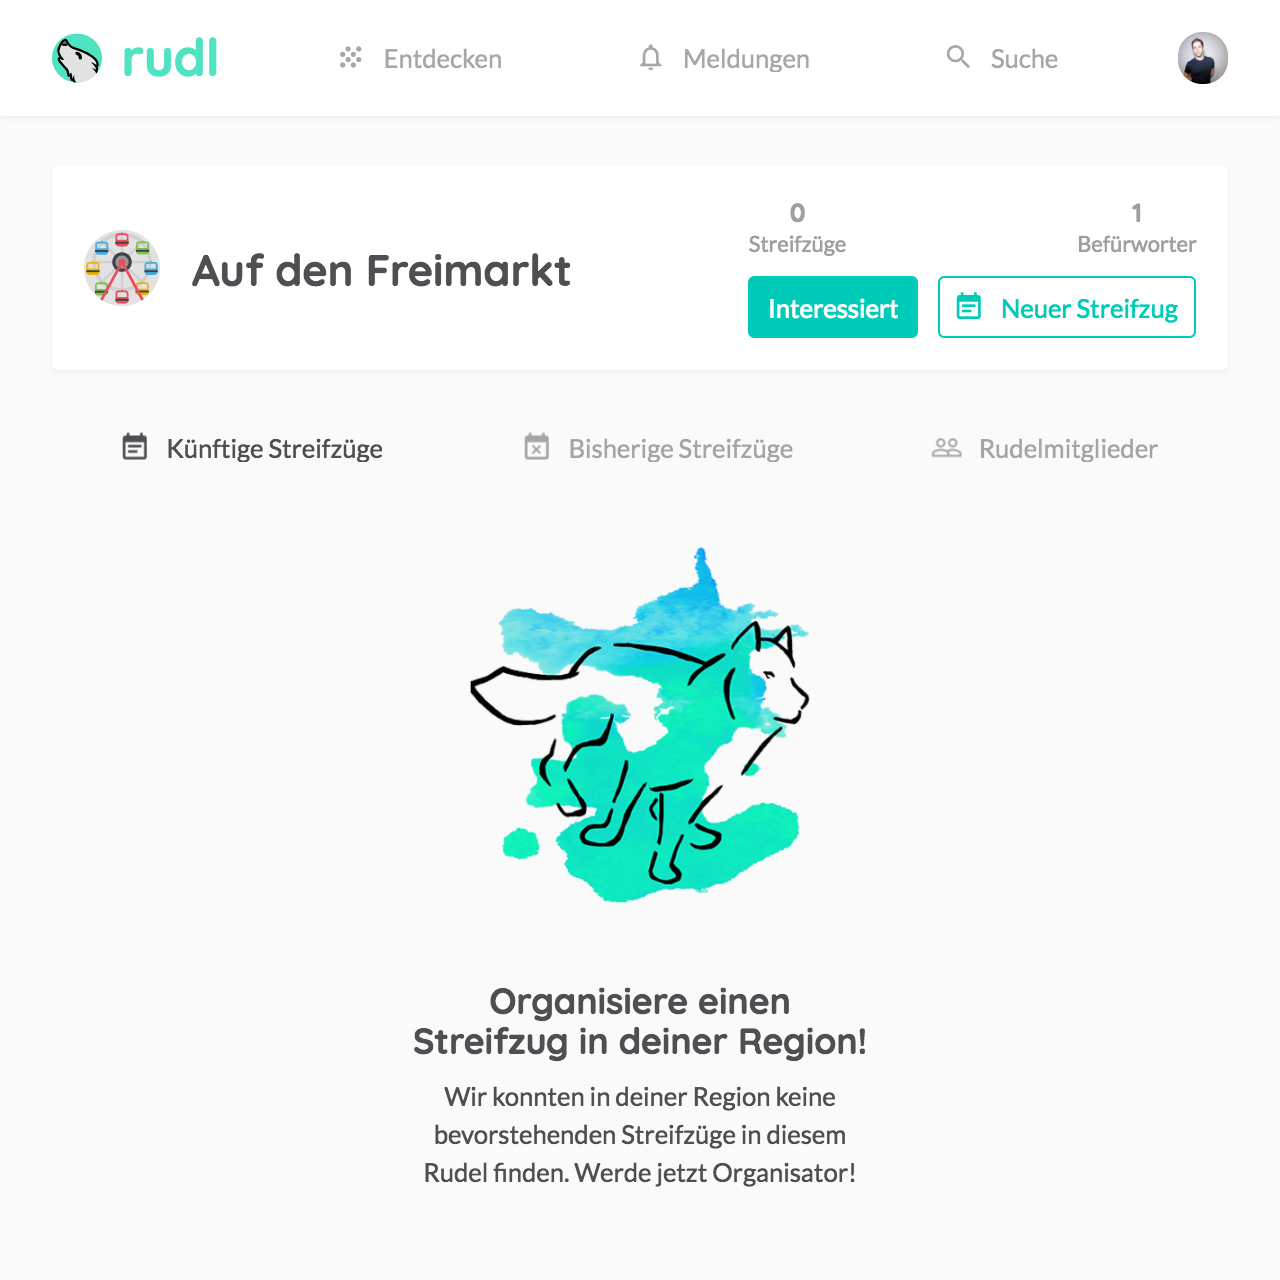
\includegraphics[width=\linewidth]{interestgroup.png}
\caption{}
\label{interestgroup}
\end{subfigure}
\caption[Organization of interest groups]{The panel of an interest group (\subref{interestgroup}) reveals important information and is accessible via the search interface (\subref{searchinterestgroup}). Interests groups are created in two steps: (\subref{createinterestgroup0}) specify a name for the interest group and (\subref{createinterestgroup1}) specify an icon for the interest group.}
\end{figure}

Joining together into interest groups is along with activities the most important objective of the application. Interest groups can consist of friends, family members or people unknown to each other. In order to let members properly find interest groups, the application should provide an easily accessible search function. Thus, the search function as shown in figure \ref{interestgroup} is shown prominently at the top of the application screen and can be activated at any time. Figure \ref{searchinterestgroup} shows an activated search function with all interest groups that are related to an entered search term. Any interest group in the list can be opened at will. 

In the case that a member is unable to find the corresponding interest group, a direct option to create one appears. In comparison to existing interest groups, the option does not come with an icon to look less attractive. This may lead to fewer duplicates and motivates everybody to select an existing interest group, if applicable. Once the option is selected, a name as shown in figure \ref{createinterestgroup0} and an icon as shown in figure \ref{createinterestgroup1} has to be set to properly create an interest group. A collection of 993 icons across seven categories shall increase the memorability and interactivity of an interest group. Once finished, the just created interest group is set as shown in figure \ref{interestgroup} and every member is able to join the group.

The panel of the interest group contains of a head area and three separate sections organized in tabs. The head area shows all important information about the interest group, including current statistics. A member can easily indicate their fellowship by clicking on the emphasized button in the head area. A list with all members of an interest group as well as lists of upcoming and past activities are shown in the corresponding section. If certain lists are empty, a placeholder with useful tips is displayed as shown in figure \ref{interestgroup}. 

\subsection{Organization of Activities}
The whole concept of the application remains in the virtual space as long as there is no way to join and create activities. Activities are accessible via the corresponding interest group as described in the previous section. 

\begin{figure}
\begin{subfigure}[t]{0.45\textwidth}
\centering
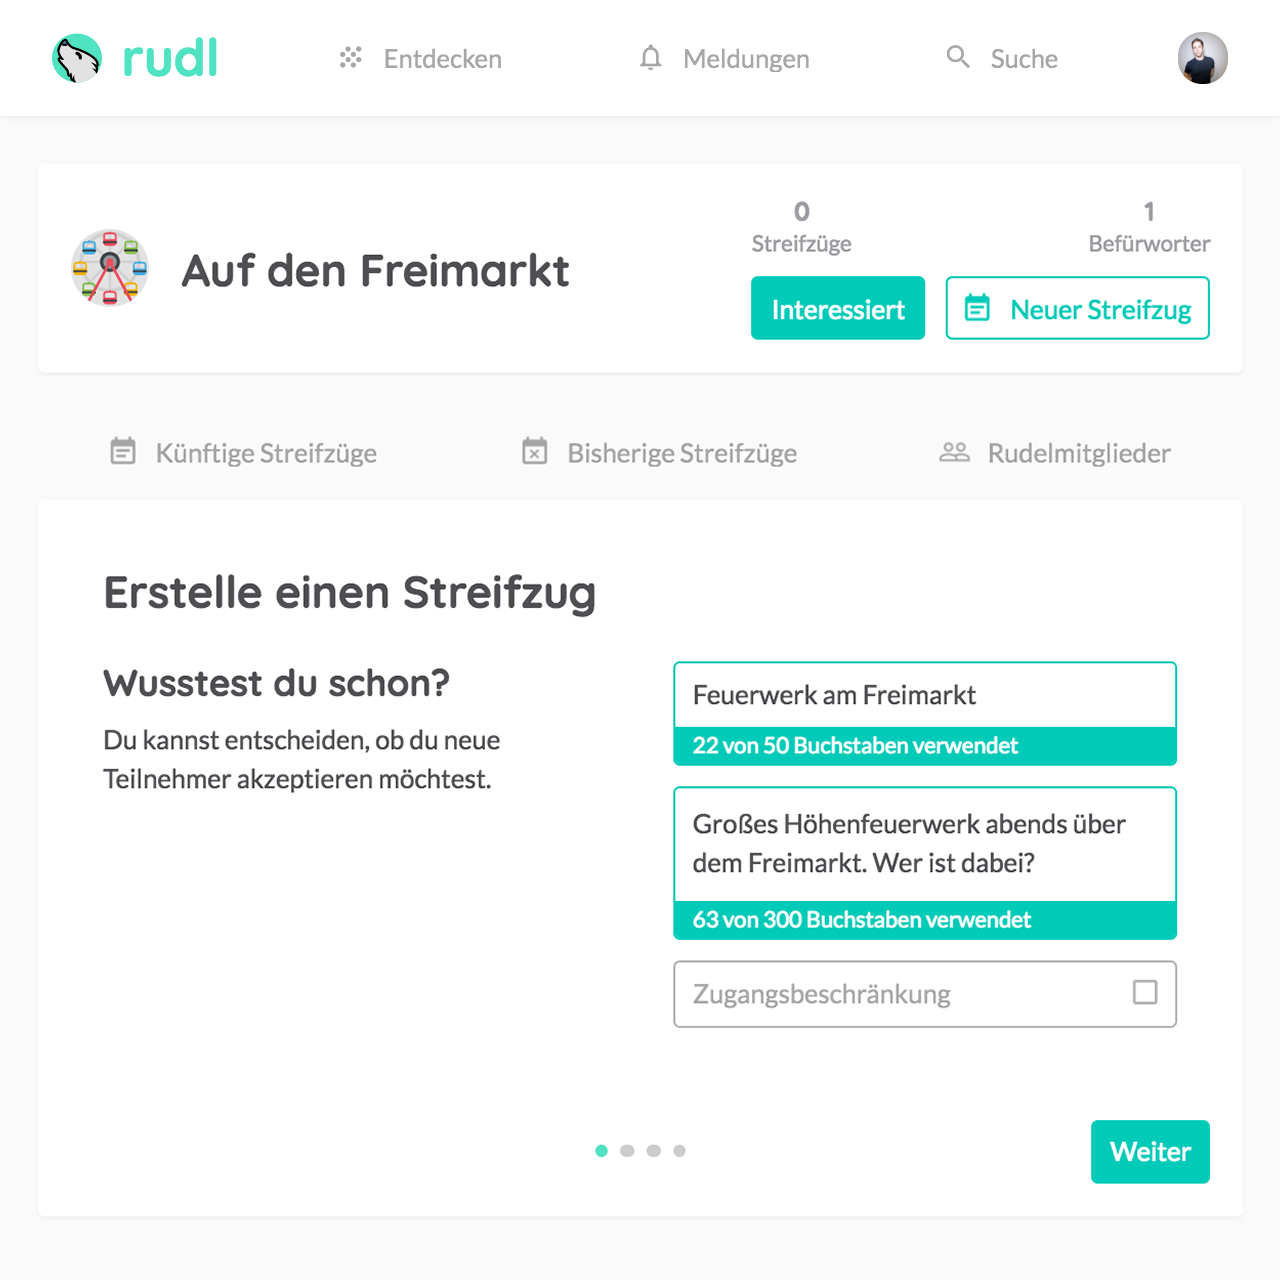
\includegraphics[width=\linewidth]{createactivity0.png}
\caption{}
\label{createactivity0}
\end{subfigure}
\hfill
\begin{subfigure}[t]{0.45\textwidth}
\centering
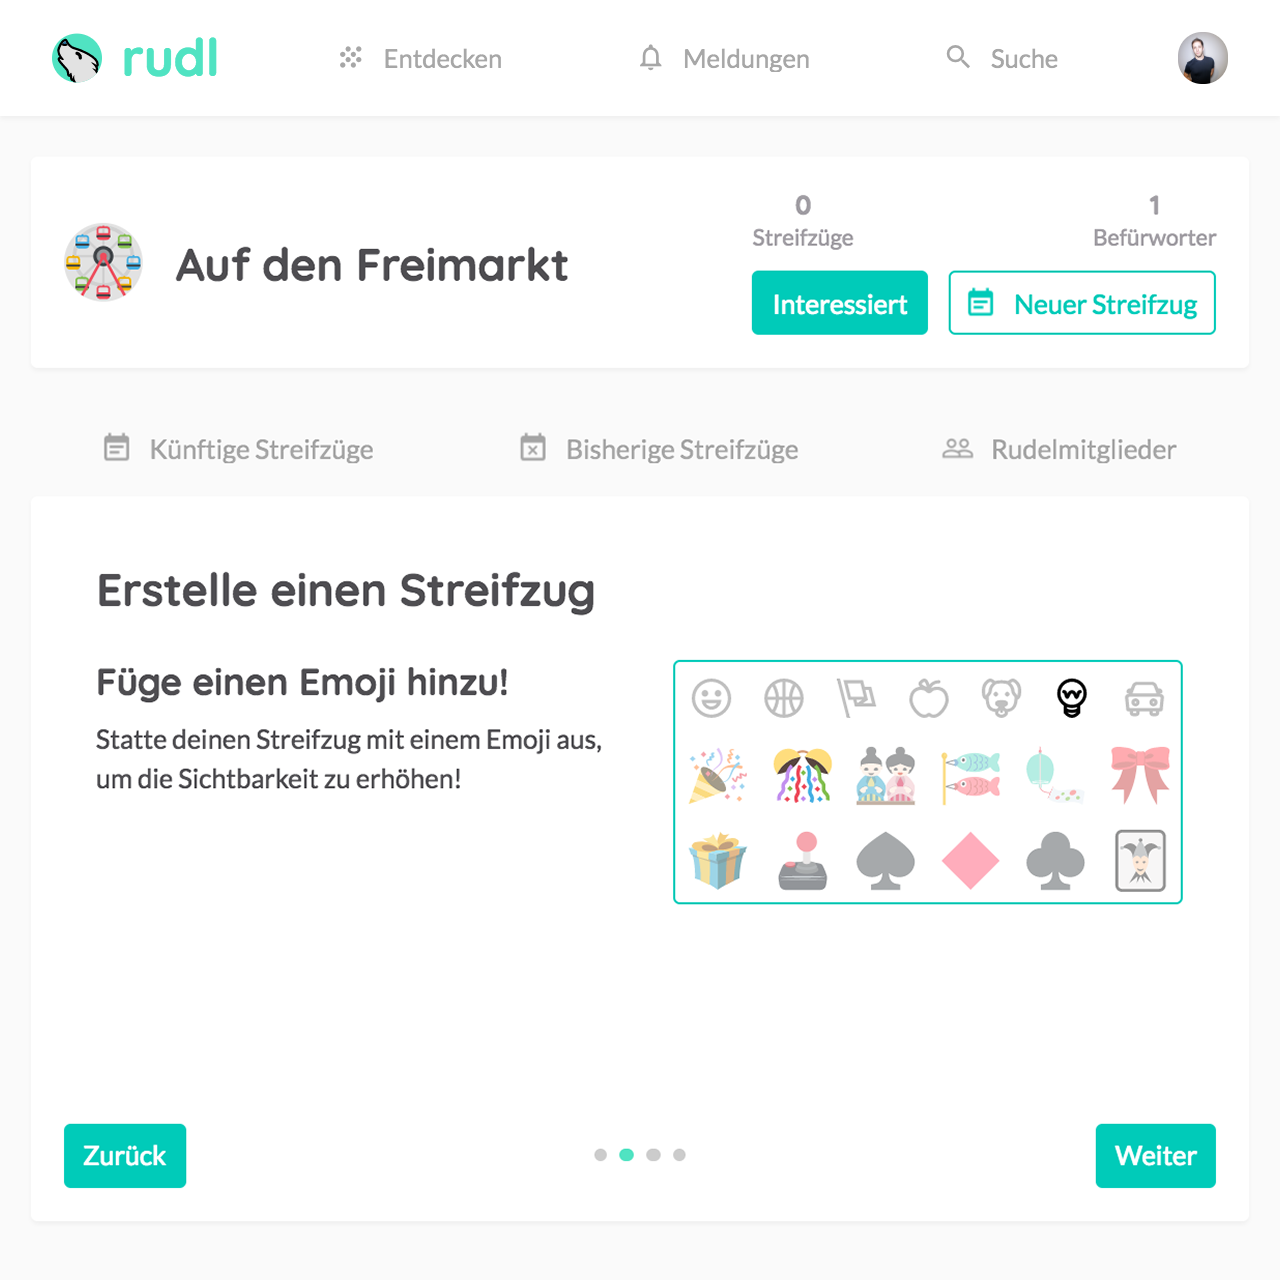
\includegraphics[width=\linewidth]{createactivity1.png}
\caption{}
\label{createactivity1}
\end{subfigure}

\bigskip

\begin{subfigure}[t]{0.45\textwidth}
\centering
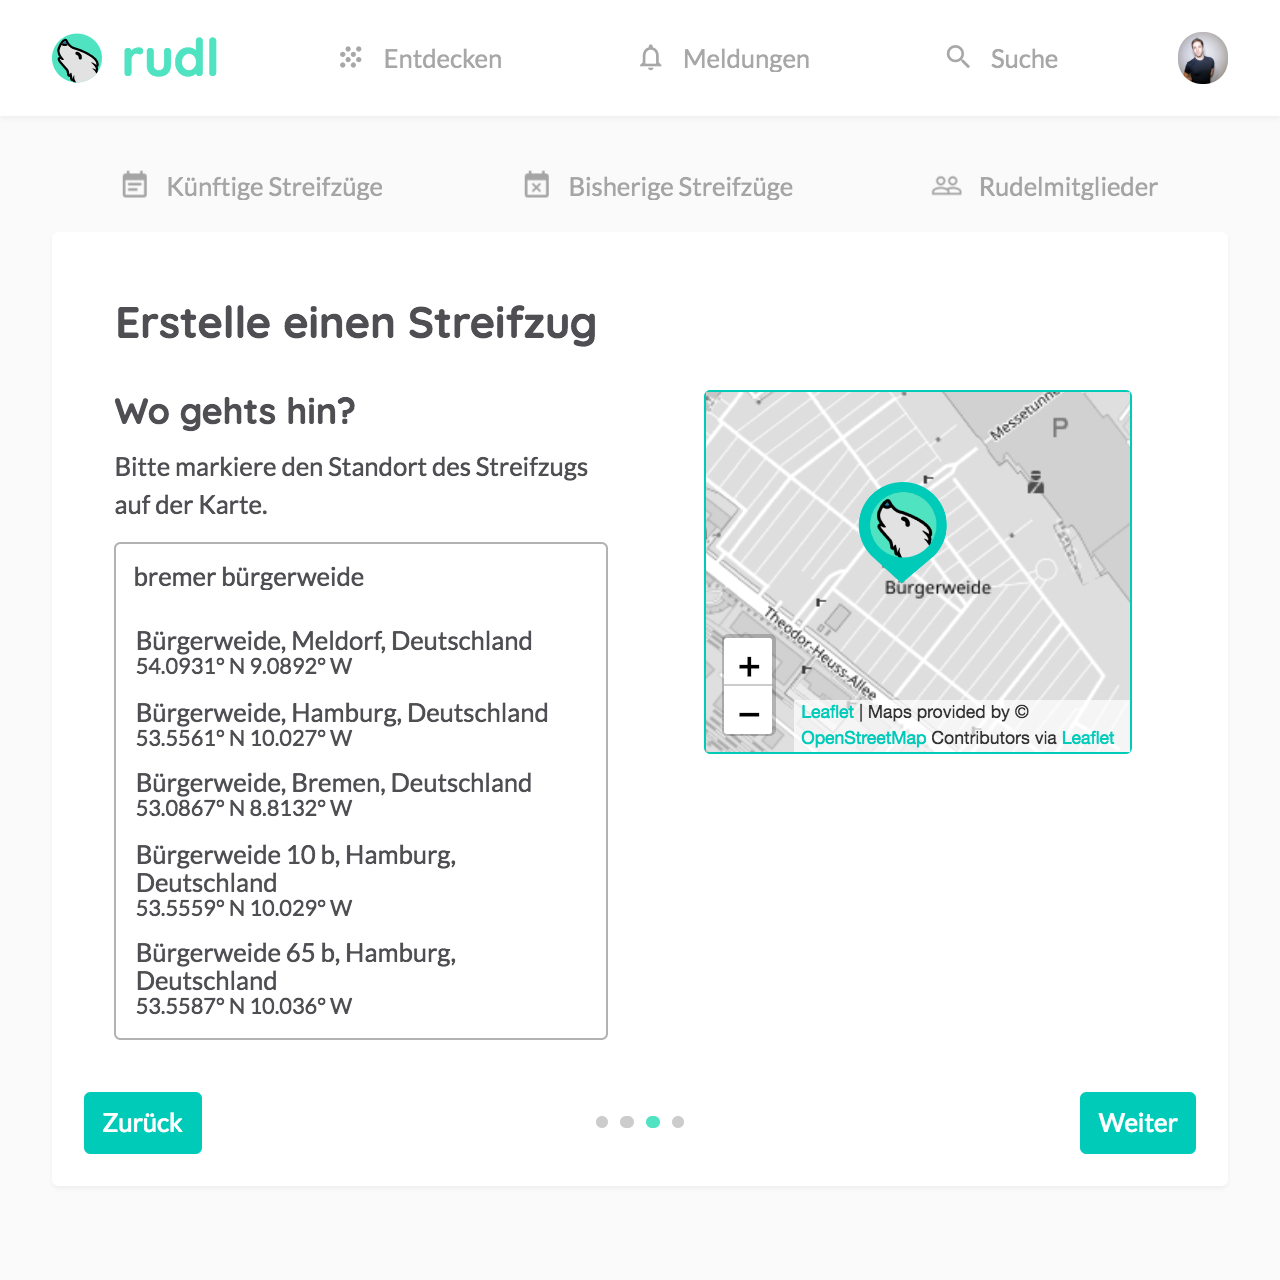
\includegraphics[width=\linewidth]{createactivity2.png}
\caption{}
\label{createactivity2}
\end{subfigure}
\hfill
\begin{subfigure}[t]{0.45\textwidth}
\centering
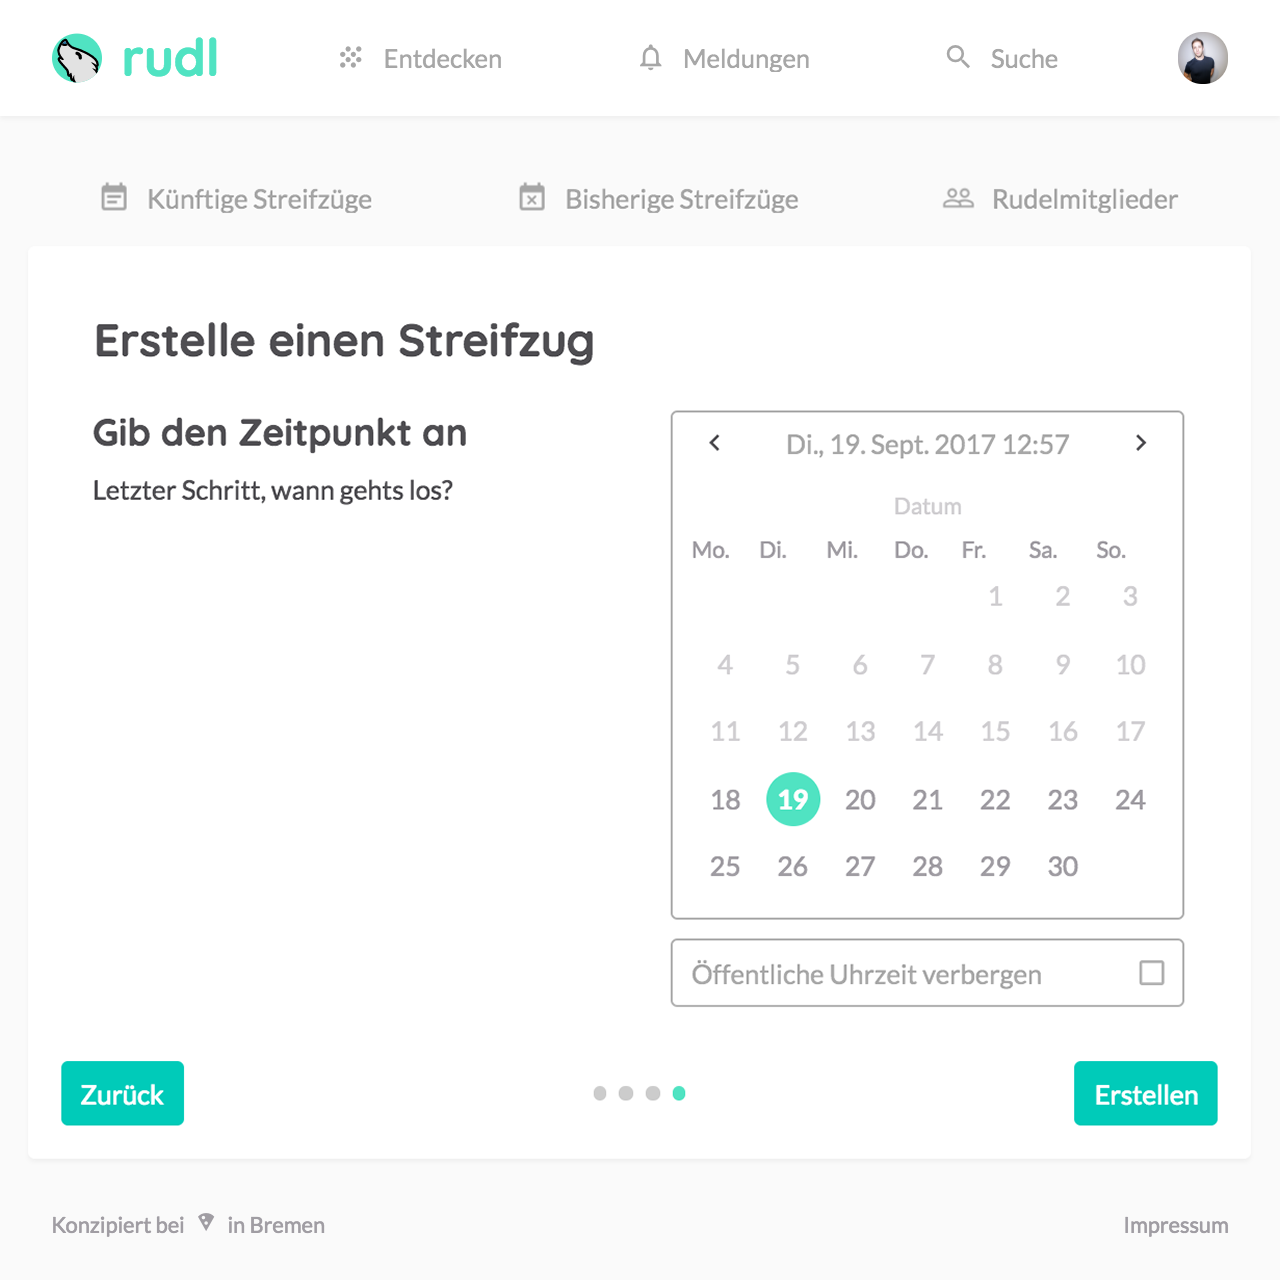
\includegraphics[width=\linewidth]{createactivity3.png}
\caption{}
\label{createactivity3}
\end{subfigure}
\caption[Creation of activities]{Creation of activities in four steps: (\subref{createactivity0}) Adjust the activity name and access control, (\subref{createactivity1}) redefine the activity icon, (\subref{createactivity2}) set the meeting point and (\subref{createactivity3}) specify date and time of the activity.}
\end{figure}

\begin{figure}
\begin{subfigure}[t]{0.45\textwidth}
\centering
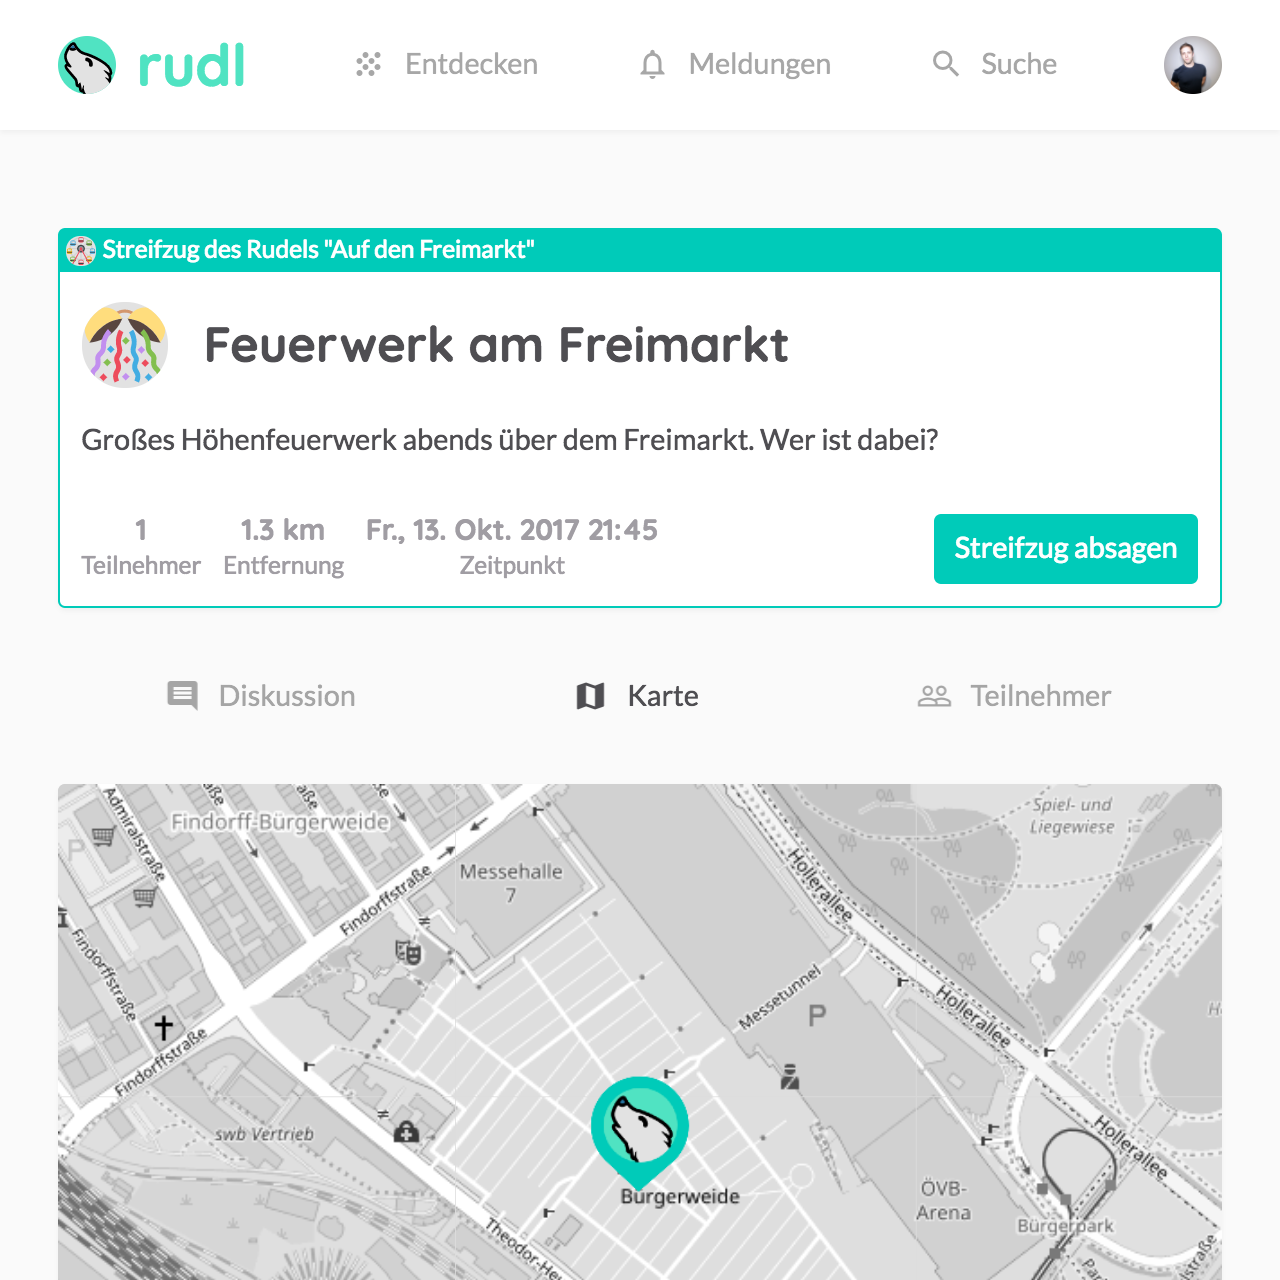
\includegraphics[width=\linewidth]{activity.png}
\caption{}
\label{activity}
\end{subfigure}
\hfill
\begin{subfigure}[t]{0.45\textwidth}
\centering
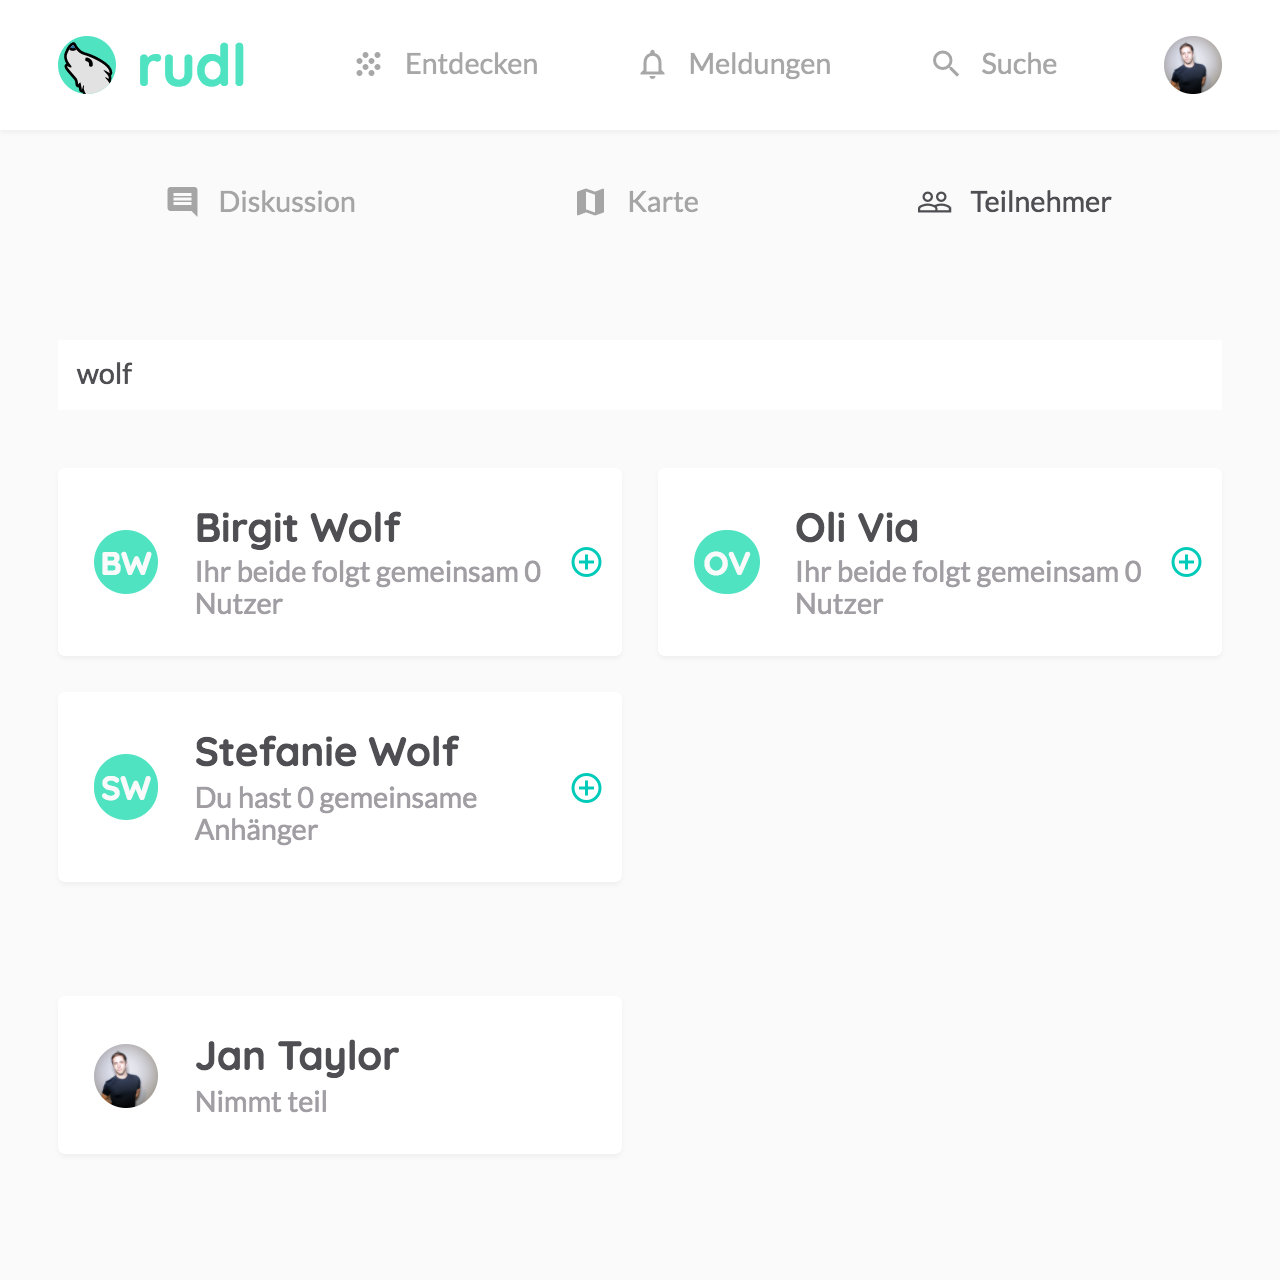
\includegraphics[width=\linewidth]{activityattendees.png}
\caption{}
\label{activityattendees}
\end{subfigure}

\bigskip

\begin{subfigure}[t]{0.45\textwidth}
\centering
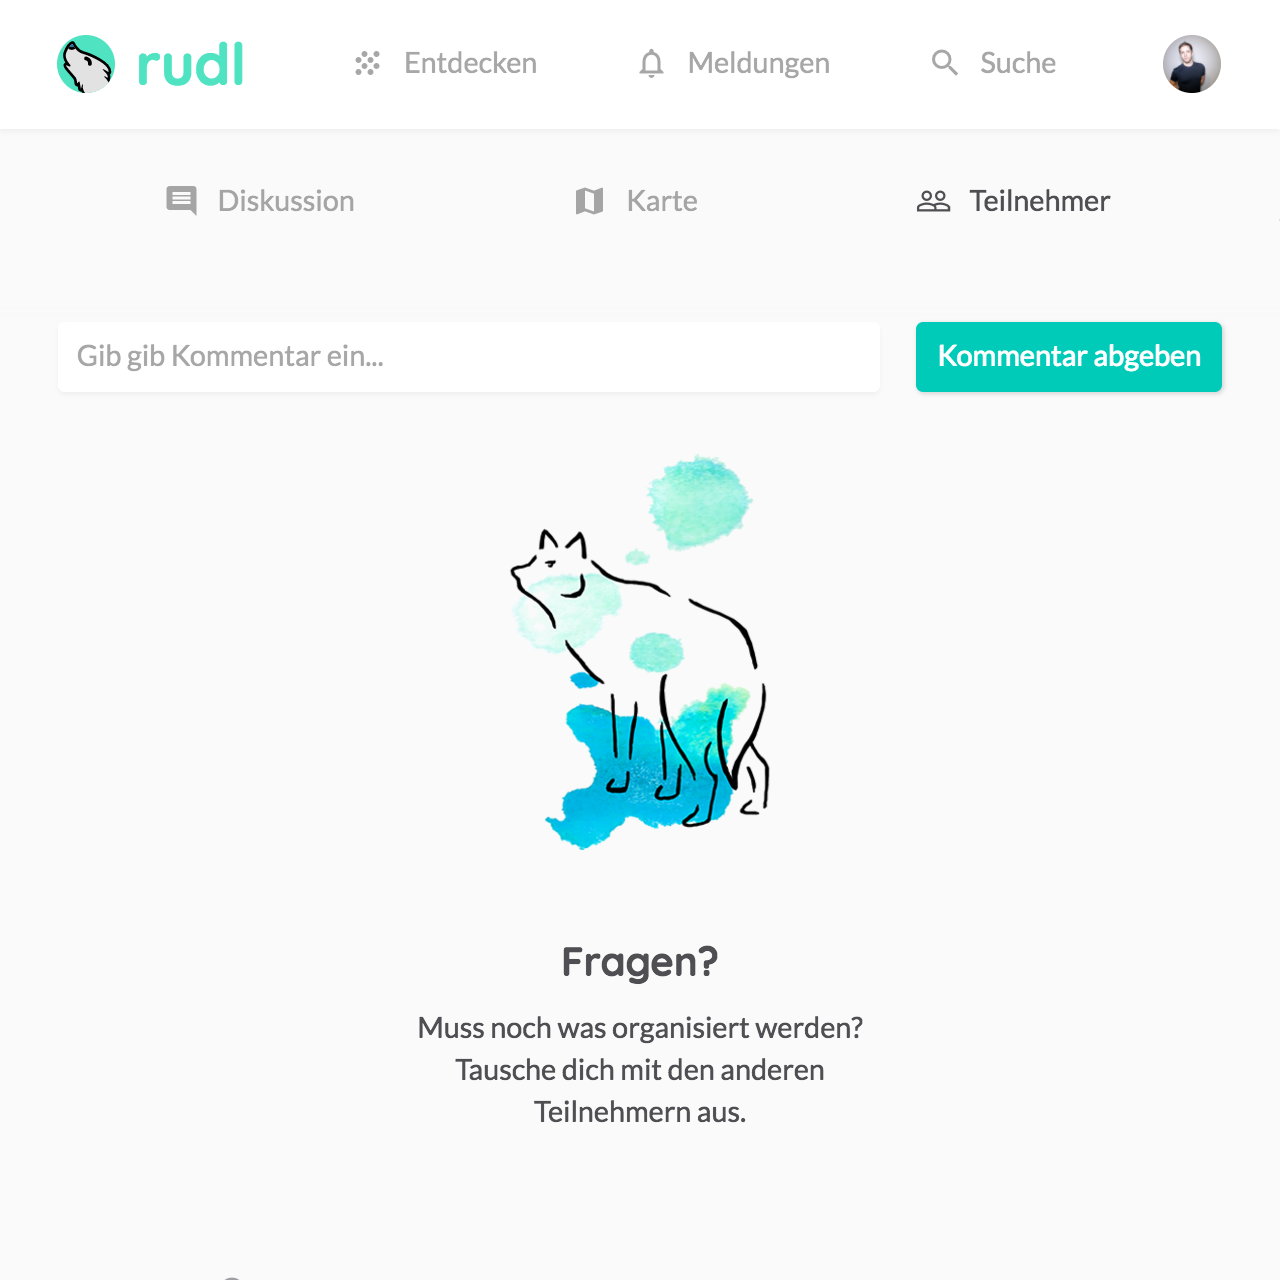
\includegraphics[width=\linewidth]{activitydiscussion.png}
\caption{}
\label{activitydiscussion}
\end{subfigure}
\hfill
\begin{subfigure}[t]{0.45\textwidth}
\centering
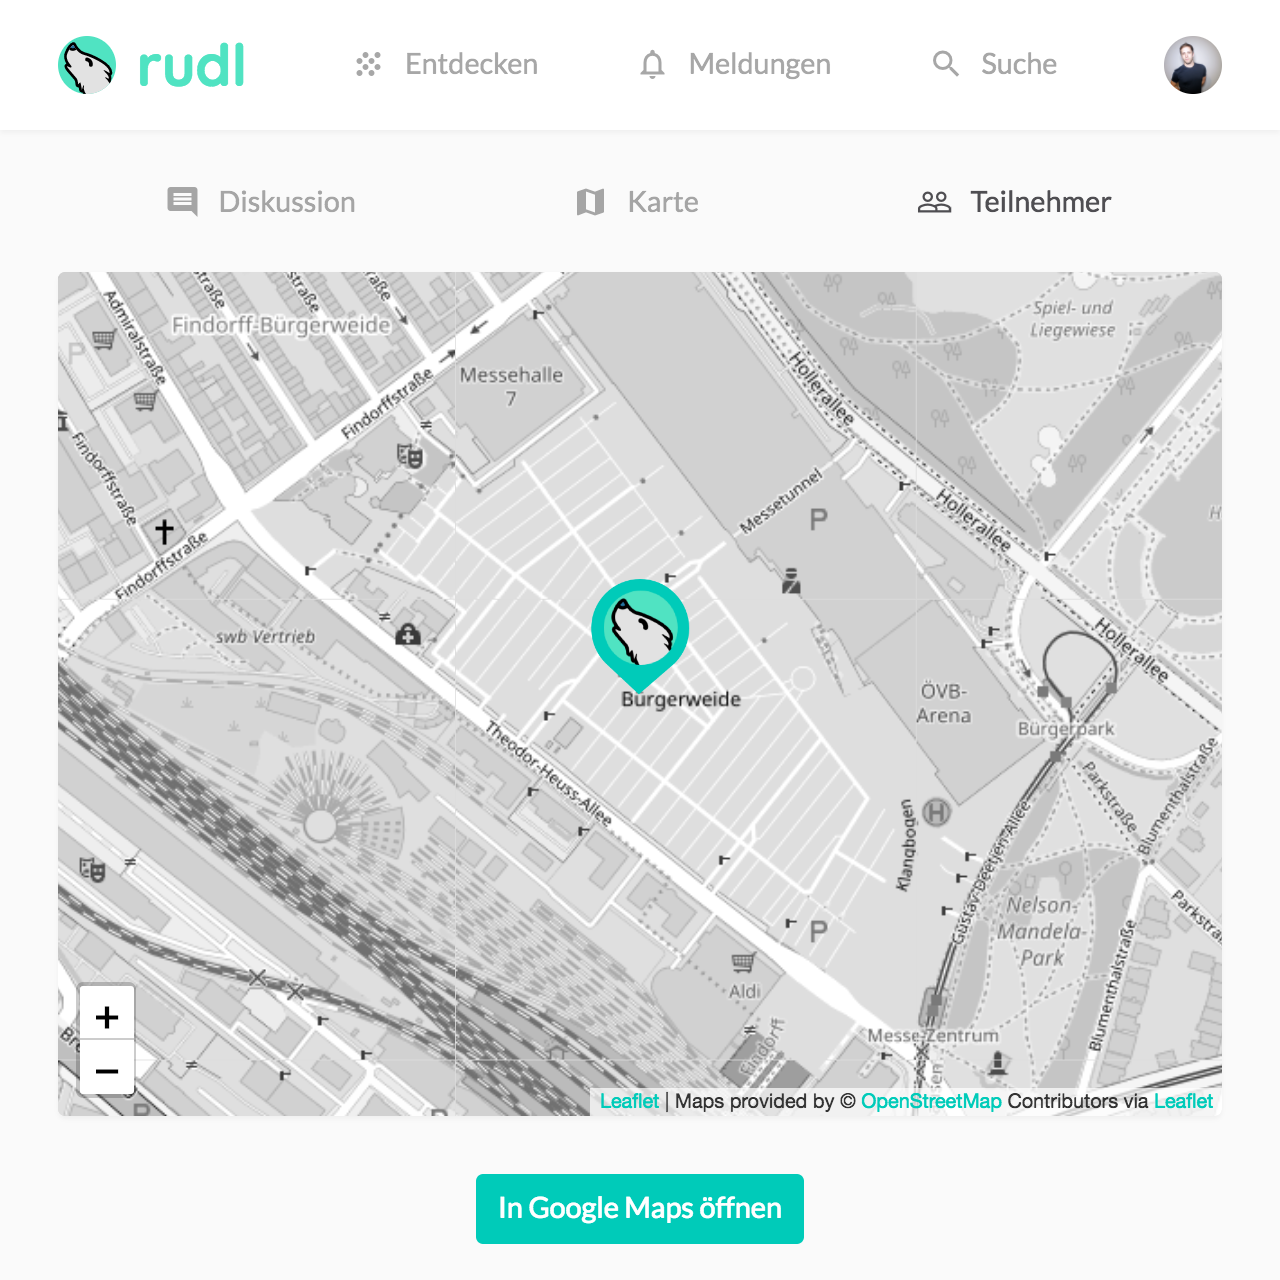
\includegraphics[width=\linewidth]{activitymap.png}
\caption{}
\label{activitymap}
\end{subfigure}
\caption[Organisation of activities]{The activity panel (\subref{activity}) comes with a map of the meeting point (\subref{activitymap}), invitation capabilities (\subref{activityattendees}) and a discussion board (\subref{activitydiscussion}) to let members plan their activity in detail.}
\end{figure}

To create an activity, a member clicks the corresponding button in the head area of the interest group and runs through four steps: At first, the member has to enter a short description, may adjust the name of the activity and turn on the access control\footnote{Activities are either freely accessible to everyone or restricted to a certain group of people. The creator may like to turn on this access control during this step. In this case, everyone interested has to apply for the participation at the activity. Once the creator has confirmed the request, the member automatically joins the activity.} as shown in figure \ref{createactivity0}. In the next step, the member has the option to adapt the icon in accordance to the chosen title of the activity. Figure \ref{createactivity1} illustrates how it is possible to change the icon accordingly. The third step as shown in figure \ref{createactivity2} displays a map to set the meeting point. In the last step, the creator sets the date and time and may decide for privacy reasons to apply an inaccuracy to the time, see figure \ref{createactivity3}.

Every activity panel is structured analogical to an interest group as it contains a head area and three separated sections. Figure \ref{activity} illustrates the head area, which displays all relevant information in order to meet in person. In the event that important information in the head area are missing, all attendees can chat with each other easily in the discussion section as shown in figure \ref{activitydiscussion}. This is the only way within the entire application to chat with each other and to make further plannings. The location section as shown in figure \ref{activitymap} comes with a large map and the ability to open third-party applications to properly navigate to the meeting point. The purpose of the last section as shown in figure \ref{activityattendees} is to invite other members to the activity. Everybody can enter the members name to send a corresponding notification. This way, it is easy to tell friends and acquaintances about the activity.

\subsection{Profile Management and Notifications}
\begin{figure}
\begin{subfigure}[t]{0.45\textwidth}
\centering
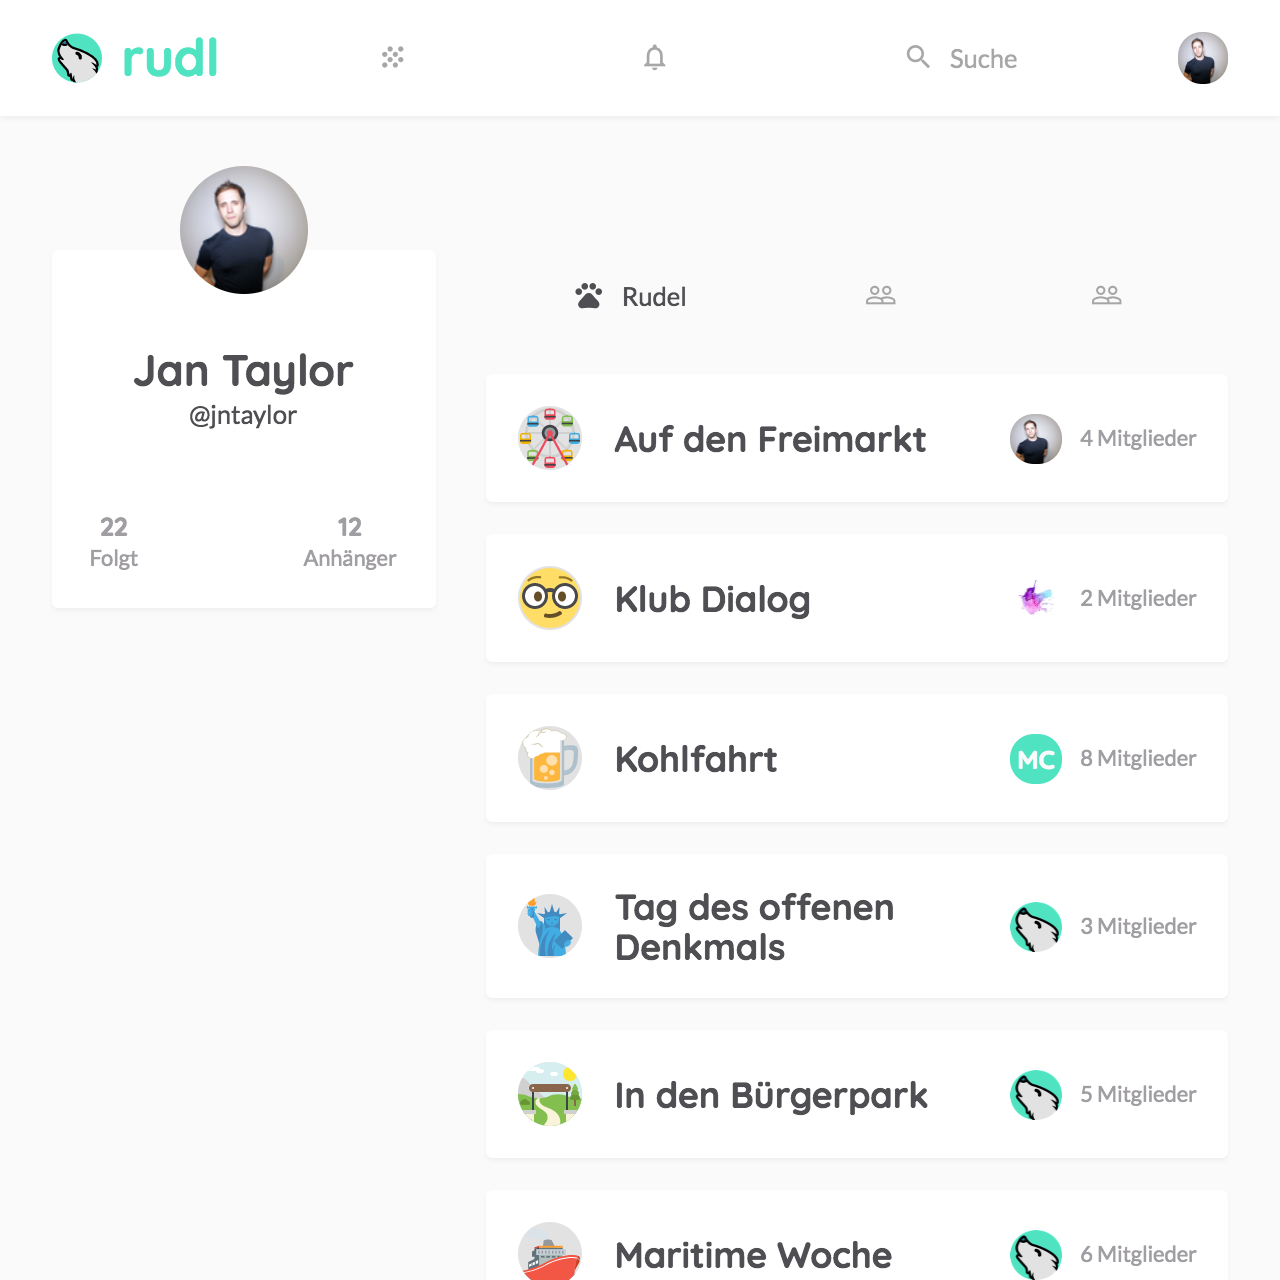
\includegraphics[width=\linewidth]{user.png}
\caption{}
\label{user}
\end{subfigure}
\hfill
\begin{subfigure}[t]{0.45\textwidth}
\centering
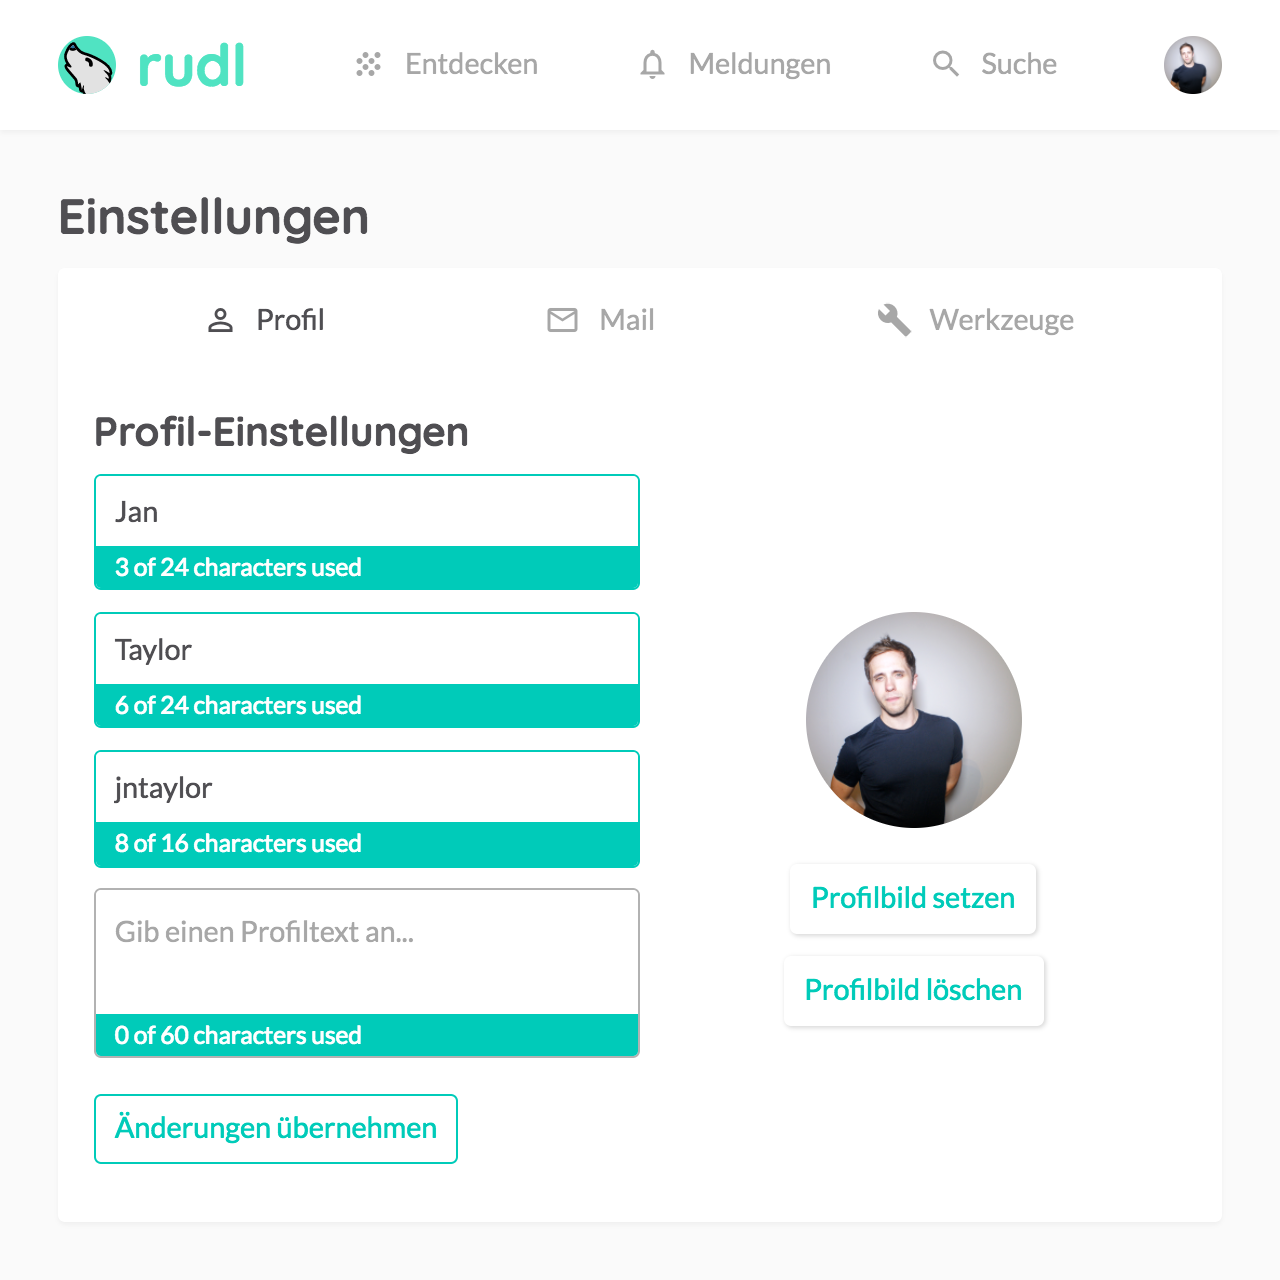
\includegraphics[width=\linewidth]{settings.png}
\caption{}
\label{settings}
\end{subfigure}

\bigskip

\begin{subfigure}[t]{0.45\textwidth}
\centering
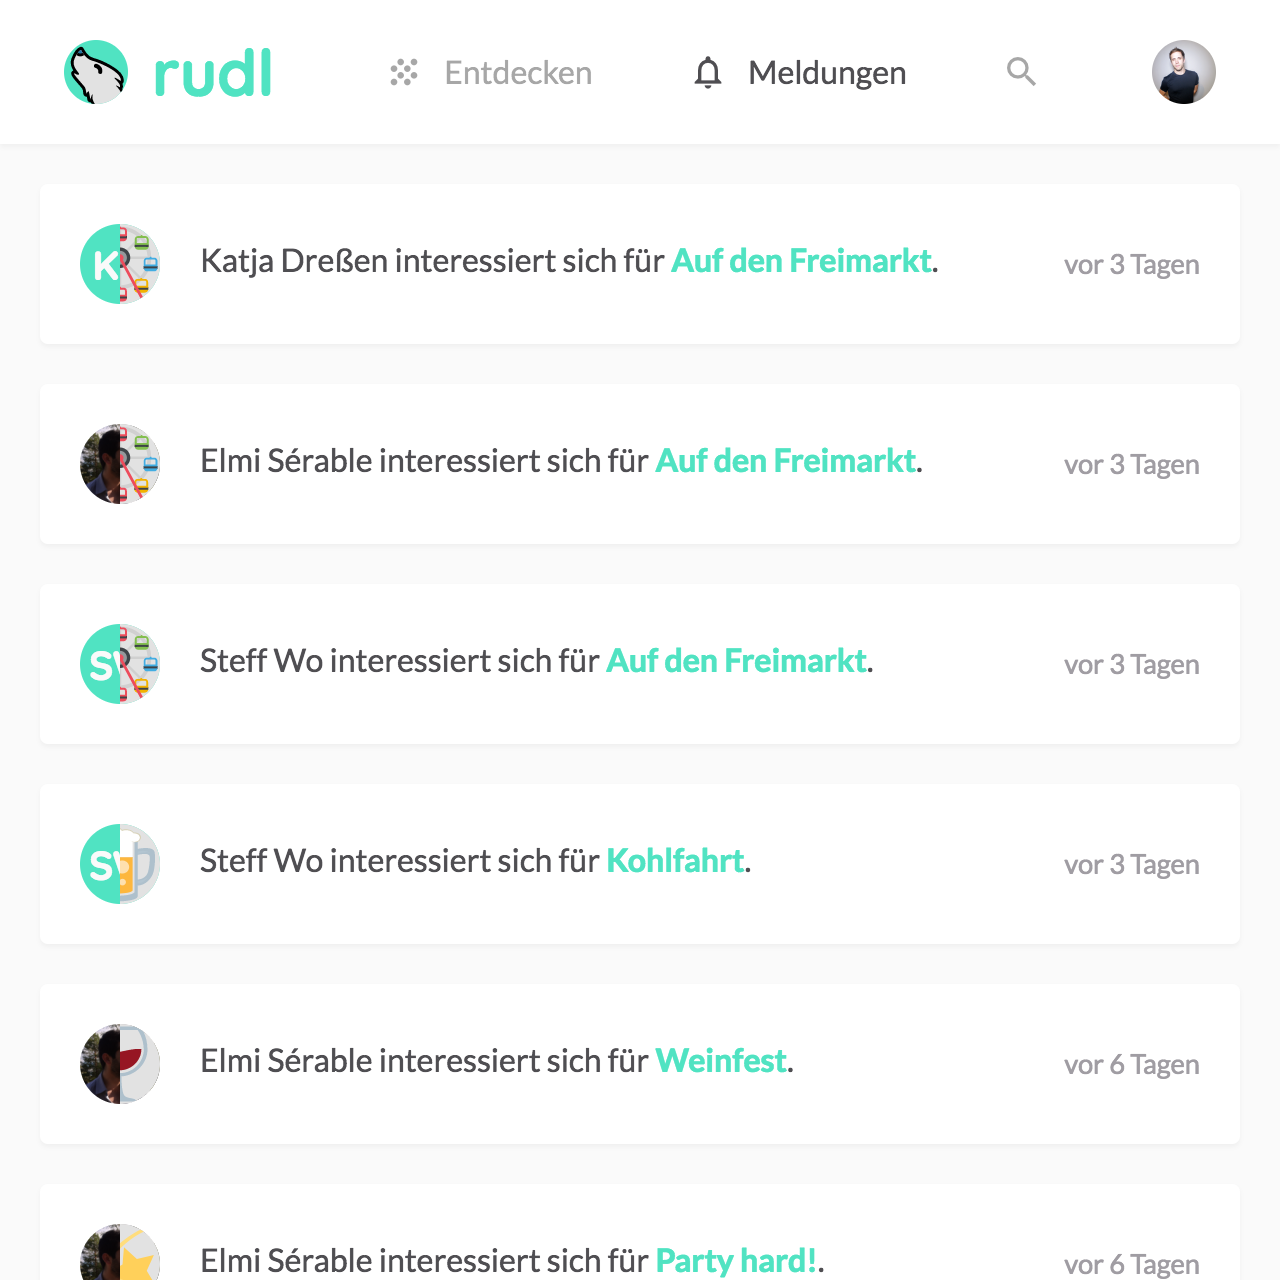
\includegraphics[width=\linewidth]{notifications.png}
\caption{}
\label{notifications}
\end{subfigure}
\hfill
\begin{subfigure}[t]{0.45\textwidth}
\centering
\includegraphics[width=\linewidth]{useractivitys.png}
\caption{}
\label{useractivitys}
\end{subfigure}
\caption[Profile Management and Notifications]{Every member has a public profile (\subref{user}), which can be configured via the settings page (\subref{settings}). Every member receives personal notifications (\subref{notifications}) as well as an overview of all joined activities (\subref{useractivitys}).}
\end{figure}

Every member in the community has a public profile that can be individualized with a picture and a short description. As shown in figure \ref{user}, every profile contains a list of all joined interest groups and an overview of all corresponding followers and followees. Members can adjust their profile within the settings page as shown in figure \ref{settings}. Additionally, the settings page allow members to delete their account or toggle notification updates via mail.

Notifications may represent a trivial principle. Carefully applied, they improve the transparency throughout the application. Members do not need to invest time to investigate wether friends, acquaintances or other related members are joining activities or started a discussion. Figure \ref{notifications} demonstrates the overview of notifications that is easily accessible via the top menu. Members will be notified as soon as one of the following events occurred:

\begin{itemize}
	\item A nearby activity had been created in one of the interest groups that the member joined.	
	\item Another member joined or left an activity that the member created.
	\item A followee of the member joined an activity that the member joined.
	\item Another member wants to join a restricted activity that the member created.
	\item The member was accepted or rejected to be attendee of a restricted activity.
	\item The member had been invited to an activity.
	\item Another member has accepted or rejected an invitation to an activity that the member created.
	\item Another member started or continued the discussion within an activity that the member joined.
	\item An activity that the member joined is scheduled for today.
	\item The member got a new follower.
	\item A followee of the member joined or created a new interest group.
\end{itemize} 

In case the member activated mail notifications via the settings page, notifications are collected on a hourly basis and sent via mail to the members inbox.

The last component in this section is an overview of all upcoming and past activities to which the member will participate or had participated. Figure \ref{useractivitys} shows the section of upcoming activities. In addition to notifications, this overview shall provide an alternative way to access all relevant activities easily.

\subsection{Explorative Components}
\begin{figure}
\begin{subfigure}[t]{0.45\textwidth}
\centering
\includegraphics[width=\linewidth]{exploreinterestgroup.png}
\caption{}
\label{exploreinterestgroup}
\end{subfigure}
\hfill
\begin{subfigure}[t]{0.45\textwidth}
\centering
\includegraphics[width=\linewidth]{exploreactivitys.png}
\caption{}
\label{exploreactivitys}
\end{subfigure}

\bigskip

\begin{subfigure}[t]{0.45\textwidth}
\centering
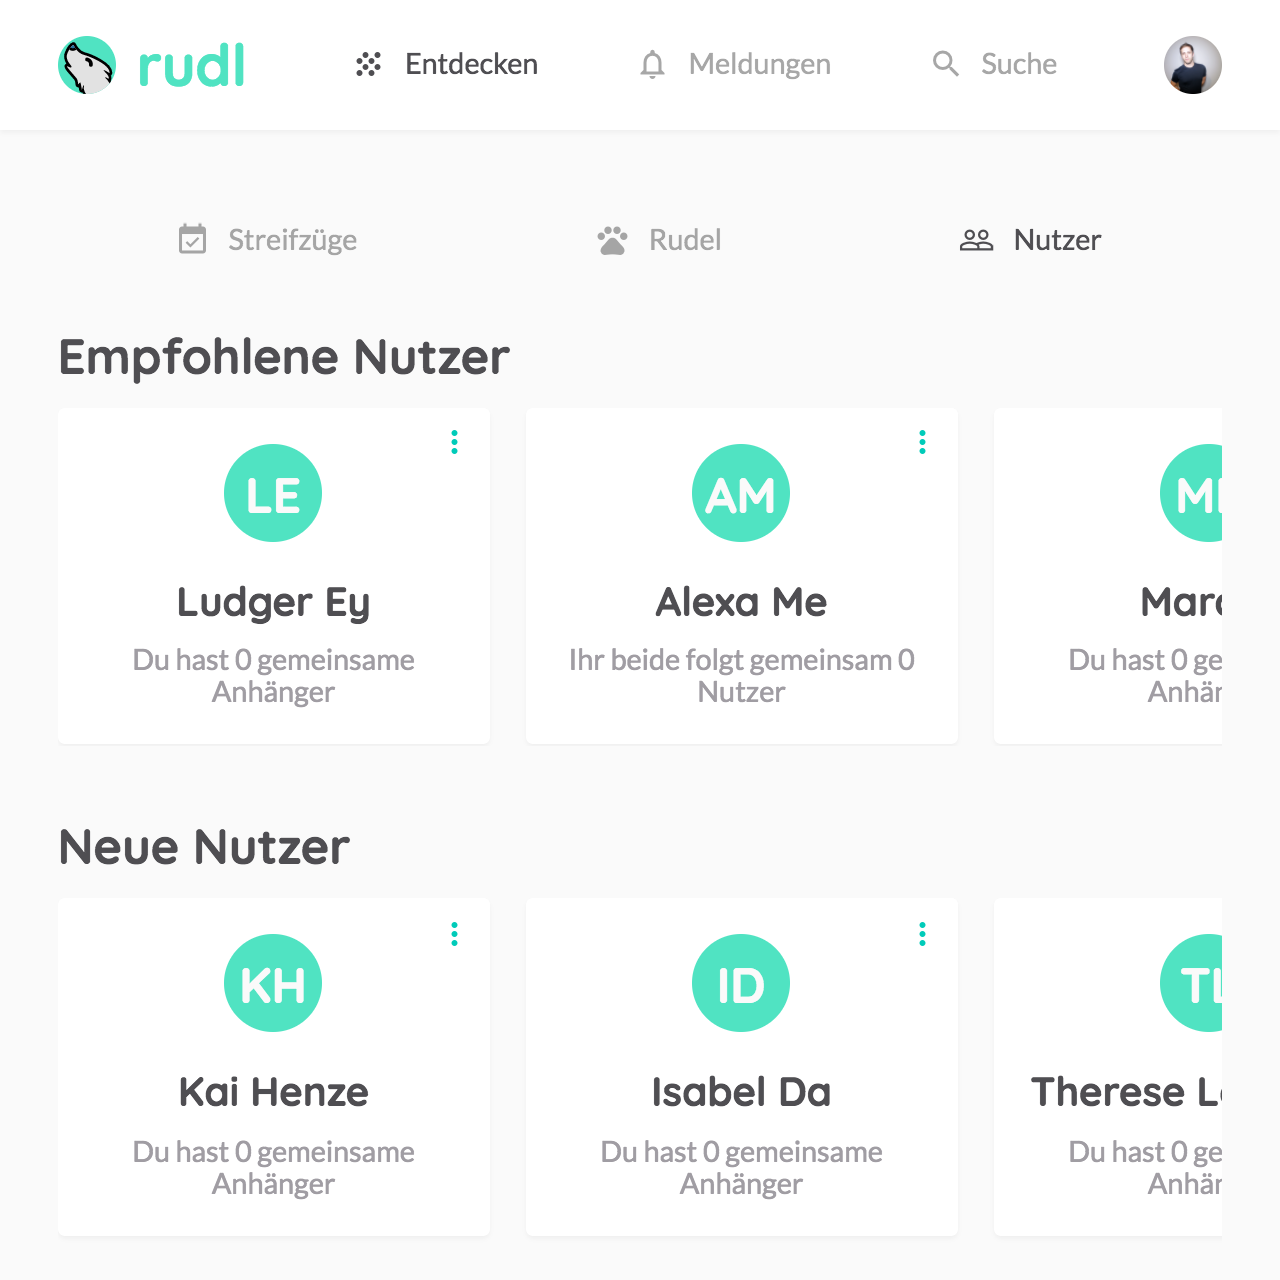
\includegraphics[width=\linewidth]{exploreusers.png}
\caption{}
\label{exploreusers}
\end{subfigure}
\caption[Explorative Components]{Explorative components either display lists of interest groups (\subref{exploreinterestgroup}), activities (\subref{exploreactivitys}) or users (\subref{exploreusers}). All lists are either sorted by popularity, recommendation quality or recency.}
\label{explore}
\end{figure}

Interest groups and activities form the foundation of the application. At present, interest groups and the related activities are accessible in a limited manner. To prevent members from having to search for new or popular interest groups and activities on their own, there has to be a feature to inform members about corresponding entries within the application. In contrast to notifications, this feature is primarily meant to address entries that the member has not yet interacted with. Similar to magazine guides, it can be convenient to browse through new and popular interest groups, activities and members. Thus, the application should provide a browsing feature that is intended to be shown right after opening the application. Figure \ref{explore} shows the exploration page, which is divided into three sections organized in tabs. Each section provides an overview of interest groups, activities or members in orders of recommendation quality, popularity and recency. The recommendations are the result of the recommendation algorithm as described in the next section.

\subsection{The Recommendation Algorithm}
Without media tools, people generally have a narrowed picture of possible leisure activities in the region. Accordingly, it is important to inform about possible leisure activities. Because of the reasons mentioned in a preceding section, the application will provide recommendations that are generated by the machine itself. As machine generated recommendations can involve far more input variables than editorially selected ones, it is possible and desirable to make recommendations on the basis of as many members, interest groups and activities as possible.

The recommendations made by the application are not meant to patronize members or take their decisions. The autonomy of all members has to be encouraged as well as their freedom to decide either to agree with a recommendation, indicate a lack of interest or fully ignore it. The algorithm should not limit this freedom or influence the final decision of a member. Otherwise, people might do something that does not correspond to their personal needs and risk stress or dissatisfaction on a long-term basis.

An analysis of every single interest group or activity describes the procedure of content based filtering. Attributes are assigned to each recommendation item to allow a comparison among all the other items \citep[p.42]{klahold2009}. Nonetheless, this implies that each member that creates an interest group or activity would have to add comprehensive descriptions of its attributes. As the number of possible attributes increases, existing recommendation elements may need to be checked and perhaps added again. This does not only require a high level of organizational work, but it would also be questionable whether members will save time. In addition, it is possible that members may provide misleading information by accident or on purpose. For this reason, it should be impossible for everybody to influence recommendations made to other members. This is why the input variables shall be exclusively based on the data provided by registered members. With this in mind, it makes sense to avoid a corresponding functionality to let members categorize interest groups and activities.\footnote{One imagines a beach club manager, who would like to promote the interest group ``Go to the beach club''. Out of this motivation, the manager decides to equip the interest group with appropriate categories indicating that activities of this particular interest group are independent from weather conditions. Clearly, this does not correspond to the truth and was chosen out of pure self-interest.} This can be done by using collaborative filtering. 

Collaborative filtering is based on the behavior of members, for example on any interest group they follow or activity they join. \citep[p.62]{klahold2009} Thereby, the algorithm does not compare the similarity of recommendation elements, but rather compares the interactions between recommendation elements and members. This can be illustrated by a member-item matrices as shown in figure \ref{matrix}.

\begin{figure}
\begin{subfigure}[t]{0.5\textwidth}
\centering
$\bordermatrix{~ & \mathit{Item_1} & \mathit{Item_2} & \mathit{Item_m} \cr
\vphantom{\vdots}\mathit{Person_1} & 1 &  & \cdots  \cr
\vphantom{\vdots}\mathit{Person_2} & 3 & 4 & \cdots \cr
\vphantom{\vdots}\mathit{Person_n} & \vdotswithin{3} & \vdotswithin{4} & \ddots  }$
\caption{}
\label{nummatrix}
\end{subfigure}%
\begin{subfigure}[t]{0.5\textwidth}
\centering
$\bordermatrix{~ & \mathit{Group_1} & \mathit{Group_2} & \mathit{Group_3} \cr
\vphantom{\vdots}\mathit{Member_1} &  & \mathit{joined} &  \cr
\vphantom{\vdots}\mathit{Member_2} & \mathit{left} & \mathit{joined} & \mathit{joined} \cr
\vphantom{\vdots}\mathit{Member_3} & &  & \mathit{joined} }$
\caption{}
\label{boolmatrix}
\end{subfigure}
\caption[Member-item matrices of collaborative filtering]{Different types of matrices as used in collaborative filtering. (\subref{nummatrix}) Numerical matrix of $m$ items and $n$ persons. (\subref{boolmatrix}) Boolean 3x3 matrix of 3 groups and 3 members.}
\label{matrix}
\end{figure}

Interactions can be compared on a multi-level scale, for instance as in movie and customer reviews, or are analysed with the help of a boolean criteria, for example to determine whether a customer has purchased a product or not. On the basis of these matrices, you can calculate corresponding similarity scores. The score indicates the similarity between two members based on their interactions. There are different calculation methods that can be used for multi-level comparisons including the euclidean distance \citep[p.75]{klahold2009}, cosine-based vector similarity \citep[p.71]{klahold2009}, the Pearson's correlation \citep[p.72]{klahold2009}, or the k-nearest neighbor \citep[p.76]{klahold2009} algorithm. Other methods support only boolean comparisons, such as the Jaccard similarity \citep[p.74]{klahold2009}. 

This application is rather simple and allows members to either show interest in a particular interest group or leave the group again. In addition, it is possible that a member did not yet interact with an interest group. For both calculation methods, it is problematic for this last case to define a certain value, like 0 or false\footnote{In a multi-level comparison, 0 could be interpreted as a bad rating, whereas false is considered negatively in a boolean comparison.} As it is fine to ignore all non-valued recommendation elements for the purpose of this application, the recommendations are made in a boolean comparison by using the Jaccard similarity. 

The Jaccard coefficient measures the similarity between two sample sets and is defined as the size of the intersection divided by the union of two finite sample sets:
\[
\mathlarger{J(\mathit{A}, \mathit{B}) = \frac{|\mathit{A} \cap \mathit{B}|}{|\mathit{A} \cup \mathit{B}|}}
\] 

Figure \ref{boolmatrix} shows an exemplary scenario in which members have interacted with different interest groups. The calculation of the Jaccard coefficient between $\mathit{Member_1}$ and $\mathit{Member_2}$ in terms of commonly joined interest groups is:
\begin{align*}
J(\mathit{Member_1}, \mathit{Member_2}) &= \frac{|\mathit{Member_1} \cap \mathit{Member_2}|}{|\mathit{Member_1} \cup \mathit{Member_2}|} \\ &= \frac{|\{\mathit{Group_2}\} \cap \{\mathit{Group_2, Group_3}\}|}{|\{\mathit{Group_2}\} \cup \{\mathit{Group_2, Group_3}\}|} = \frac{|\{\mathit{Group_2}\}|}{|\{\mathit{Group_2, Group_3}\}|} \\ &= 0.5
\end{align*}
In order to recommend $\mathit{Member_1}$ matching interest groups, the similarity between $\mathit{Member_1}$ and all other members has to be calculated. $\mathit{Member_3}$ receives a coefficient of $0$ and is therefore ranked behind $\mathit{Member_2}$. The next step is to sort all other members in a descending order by their coefficients. In this sequence, all joined interest groups of every member are collected that have never got the attention of $\mathit{Member_1}$. As soon as the requested number of recommendations has been reached, the process stops and the corresponding recommendations can be displayed. In this particular scenario, $\mathit{Group_3}$ is going to be the top item in this list.

\begin{figure}
\begin{subfigure}[t]{\textwidth}
\centering
\begin{tikzpicture}[table/.style={matrix of nodes, nodes in empty cells, nodes = {rectangle, anchor = center, minimum height = 1.25em, font = \sffamily, text height = 1.5ex, text depth = .25ex, align = center, draw}}]

\matrix(activity) [table, label = above:Activity, text width = 3em, column 1/.style = {nodes = {text width = 1.5em}}] {id & name\\0 & Act1\\1 & Act2\\};

\matrix(member) [table, label = above:Member, text width = 3em, right = .5em of activity, column 1/.style = {nodes = {text width = 1.5em}}] {id & name\\0 & Kim \\1 & Alex\\};

\matrix(group) [table, label = above:Group, left = .5em of activity, text width = 3em, column 1/.style = {nodes = {text width = 1.5em}}] {id & name\\0 & Grp1\\};
    
\matrix(interestedin) [table, label = below:INTERESTED\_IN, below = 5em of activity, text width = 4.5em, column 1/.style = {nodes = {text width = 3em}}] {group & member\\0 & 0\\0 & 1\\};
    
\matrix(belongsto) [table, label = below:BELONGS\_TO, left = .5em of interestedin, text width = 5.5em, column 1/.style = {nodes = {text width = 3em}}] {group & activity\\0 & 0\\0 & 1\\};

\matrix(joinsactivity) [table, label = below:JOINS\_ACTIVITY, right = .5em of interestedin, text width = 5.5em] {member & activity\\0 & 1\\1 & 0\\};

\draw[thick] (group-2-1.south)--++(-.5em,-2.75em)-|(belongsto-1-1.north);
\draw[thick] (group-2-1.south)--++(.5em,-2.75em)-|(interestedin-1-2.north);
\draw[thick] (activity-3-1.south)--++(-.5em,-3em)-|(belongsto-1-2.north);
\draw[thick] (activity-3-1.south)--++(.5em,-3em)-|(joinsactivity-1-2.north);
\draw[thick] (member-3-1.south)--++(-.5em,-4em)-|(interestedin-1-1.north);
\draw[thick] (member-3-1.south)--++(.5em,-4em)-|(joinsactivity-1-1.north);
\end{tikzpicture}
\caption{}
\label{relationaldatabase}
\end{subfigure}

\bigskip

\begin{subfigure}[b]{\textwidth}
\centering
\begin{tikzpicture}[ >= stealth', shorten >= 1pt, node distance = 15em, on grid, every text node part/.style = {align = center}]
 	\node[state] (g0) {Group\\ \textit\small{id: 0}\\ \textit\small{name: Grp1}};  
	\node[state] (m1) [above right = of g0] {Member\\ \textit\small{id: 1}\\ \textit\small{name: Alex}};
 	\node[state] (a0) [below right = of g0] {Activity\\ \textit\small{id: 0}\\ \textit\small{name: Act1}};
 	\node[state] (a1) [below left= of g0] {Activity\\ \textit\small{id: 1}\\ \textit\small{name: Act2}};
 	\node[state] (m0) [above left = of g0] {Member\\ \textit\small{id: 0}\\ \textit\small{name: Kim}};
	\path[->, thick] (m0) edge node[fill = white, inner sep = 3pt] {INTERESTED\_IN} (g0);
	\path[->, thick] (m1) edge node[fill = white, inner sep = 3pt] {INTERESTED\_IN} (g0);
	\path[->, thick] (a0) edge node[fill = white, inner sep = 3pt] {BELONGS\_TO} (g0);
	\path[->, thick] (a1) edge node[fill = white, inner sep = 3pt] {BELONGS\_TO} (g0);
	\path[->, thick] (m0) edge node[fill = white, inner sep = 3pt] {JOINS\_ACTIVITY} (a1);
	\path[->, thick] (m1) edge node[fill = white, inner sep = 3pt] {JOINS\_ACTIVITY} (a0);
\end{tikzpicture}
\caption{}
\label{graph database}
\end{subfigure}%
\caption[Comparison of relational and graph databases]{Comparison of relational and graph databases.}
\label{databases}
\end{figure}

In relational databases, many database tables have to be iterated to model the complex relationships between members, interest groups and activities. In this way, database queries are more error-prone and may require an unoptimized number of computational operations.
This use case is well suited for graph databases as they can represent members, interest groups and activities as nodes and relationships as edges. The graph database resolves all relationships without the help of the programmer and uses optimized algorithms to keep the number of computational operations as small as possible. Manual iterations across multiple database tables are no longer necessary. Figure \ref{databases} compares two exemplary models that represent two members, who are interested in one interest group and participate in separate activities. The graph model clearly increases the clarity.

The graph database Neo4j \citep{neo4j} is one of the most known graph database and allows to perform database queries in a query language called Cypher. Nodes and edges are represented in round and square brackets and are linked using hyphens. Figure \ref{recommendationalogirthminterestgroups} shows the final version of the commented database query in Cypher to recommend ten interest groups to a member based upon the Jaccard similarity.

\begin{figure}
\centering
\begin{lstlisting}
// Find all users that have at least one joined interest group in common with u1.
MATCH (u1:User {id: $userId})-[:LIKES_RUDEL]->(intersection:Rudel)<-[:LIKES_RUDEL]-(u2:User) 
WHERE u2 <> u1 

// For every user: Count the number of joined interest groups that the corresponding user has in common with u1.
WITH u1, COUNT(DISTINCT intersection) AS intersection, u2 

// Retrieve and transform all joined interest groups of u1 and the corresponding user to sample sets.
MATCH (rudel_u1:Rudel)<-[:LIKES_RUDEL]-(u1), (u2)-[:LIKES_RUDEL]->(rudel_u2:Rudel) 
WITH COLLECT(DISTINCT rudel_u1) AS rudel_u1, u1, intersection, u2, COLLECT(DISTINCT rudel_u2) AS rudel_u2 

// Take the union of both sample sets.
WITH u1, LENGTH(rudel_u1 + filter(x IN rudel_u2 
WHERE NOT x IN rudel_u1)) AS union, intersection, u2 

// Calculate the Jaccard coefficient of u1 and the corresponding user. 
WITH TOFLOAT(intersection) / union AS similarity, u1, u2 

// Order all users by their coefficient.
ORDER BY similarity DESC 

// In this sequence, find the ten topmost interest groups that the corresponding users had joined, but got no attention by u1.
MATCH (r:Rudel)<-[:LIKES_RUDEL]-(u2) 
WHERE NOT (r)<-[:LIKES_RUDEL]-(u1) AND NOT (r)<-[:DISLIKES_RUDEL]-(u1) 
WITH DISTINCT r 
LIMIT 10
RETURN r
\end{lstlisting}
\caption[Algorithm to recommend interest groups]{The entire algorithm to recommend interest groups to a particular member.}
\label{recommendationalogirthminterestgroups}
\end{figure}

In the same way, other members are recommended to a particular member as shown in figure \ref{recommendationalogirthmmembers}. In contrast to the previous algorithm, the list of recommended members is returned without further processing and only consist of members that got no attention by the corresponding member.

\begin{figure}
\centering
\begin{lstlisting}
// Find all users that got no attention by u1 and joined at least one interest group commonly.
MATCH (u1:User {id: $userId})-[:LIKES_RUDEL]->(intersection:Rudel)<-[:LIKES_RUDEL]-(u2:User) 
WHERE u2 <> u1 AND NOT (u1)-[:LIKES_USER|:DISLIKES_USER]->(u2) 

// For every user: Count the number of joined interest groups that the corresponding user has in common with u1.
WITH u1, COUNT(DISTINCT intersection) AS intersection, u2 

// Retrieve and transform all joined interest groups of u1 and the corresponding user to sample sets.
MATCH (rudel_u1:Rudel)<-[:LIKES_RUDEL]-(u1), (u2)-[:LIKES_RUDEL]->(rudel_u2:Rudel) 
WITH COLLECT(DISTINCT rudel_u1) AS rudel_u1, u1, intersection, u2, COLLECT(DISTINCT rudel_u2) AS rudel_u2 

// Take the union of both sample sets.
WITH u1, LENGTH(rudel_u1 + filter(x IN rudel_u2 
WHERE NOT x IN rudel_u1)) AS union, intersection, u2 

// Calculate the Jaccard coefficient of u1 and the corresponding user. 
WITH TOFLOAT(intersection) / union AS similarity, u1, u2 

// Return the ten topmost users in the order of their coefficient.
ORDER BY similarity DESC 
LIMIT 10
RETURN u2
\end{lstlisting}
\caption[Algorithm to recommend members]{The entire algorithm to recommend members to a particular member.}
\label{recommendationalogirthmmembers}
\end{figure}

\begin{figure}
\centering
\begin{lstlisting}
// Retrieve the nearest activities within the distance of 0.5 kilometers to u.
MATCH (u:User {id: $user.id})
WITH u CALL spatial.closest("Expedition", $user.location, 0.5) YIELD node AS e 
WITH e, u 

// Keep only the activities that belong to a joined interest group of u and are dated within the next seven days.
WHERE (e)-[:BELONGS_TO_RUDEL]->(:Rudel)<-[:LIKES_RUDEL]-(u) AND NOT (e)<-[:JOINS_EXPEDITION]-(u) AND e.date > TIMESTAMP() AND e.date < TIMESTAMP() + 604800 
WITH e

// Return the ten topmost recent activities.
ORDER BY e.date 
LIMIT 10
RETURN e
\end{lstlisting}
\caption[Algorithm to recommend activities]{The entire algorithm to recommend activities to a particular user.}
\label{recommendationalogirthmactivitys}
\end{figure}

While interest groups are location-independent, activities are associated with a geographical location. In order to recommend activities to a particular member, it is now necessary to add attention to their individual location. For this reason, activities can be determined using element-based filtering. With this in mind, all activities are gathered that belong to at least one interest group of the particular member and are scheduled within the next seven days in a radius of 30 kilometers. The activities are sorted in ascending order of date. The distance can be calculated easily as shown below:
\[
\mathlarger{D(x_1, y_1, x_2, y_2) = \sqrt{(\Delta x)^2+(\Delta y)^2}}
\]
With a small number of activities, the computing costs to calculate all distances will not be high. To ensure that the algorithm remains performant for a large number of activities, it is advisable to sort the activities by their geographical location in an R-tree structure. Each node within the tree defines a geographic rectangle that is becoming more and more specific as its level increases. Activities are placed as leaf nodes at the respective nodes. Now, it is easy to determine all activities within a certain radius. Starting from the root, all the nodes are ignored whose geographical rectangle does not intersect with the query circle. Finally, all remaining leaf nodes are collected and returned.

The Spatial Plugin \citep{spatial} for Neo4j can be installed to handle this process automatically without the necessity of special programming. Figure \ref{recommendationalogirthmactivitys} shows the commented database query to recommend relevant activities to a member and also illustrates the usage of the plugin. 

With the algorithms presented here, tendential predictions can be made. Nevertheless, the algorithms are still simple and abusive actions cannot be detected by the algorithm itself. Similar member profiles can be created to make use of the collaborative filtering method to influence recommendations made to a particular member. It is also possible to specify the location and interest group of an activity in such a way that potential recommendations may reach people of a certain neighbourhood and interest.

Besides potential abuse, no additional precautions have been made to avoid filter bubbles\footnote{Filter bubbles occur as soon as people are solely surrounded by items they like due to personalized algorithms.} and cold start problems\footnote{The cold start describes a problem that occurs as soon as a system cannot cannot make reliable inferences due to insufficient interaction data.} along made recommendations.

\section{Required Hardware and Software}
The complexity of the application is extremely challenging and the implementation by a single person cannot be completed in a predictable time. Solely the co-action of multiple third-party components and the integration of the individual implementation, makes it possible to oversee and operate such a complex system. Thus, this section gives an overview explaining the rough infrastructure of hardware and software for the entire application as shown in figure \ref{application}.

The first major component is the web server that is required to store and execute the corresponding database and the program code. In theory, the location of a web server is irrelevant as long as the location provides a reliable connection to the internet. Due to privacy concerns, it is desirable to use a web server located inside Germany. The second major component are all the devices that belong to members and are equipped with modern browsers. These clients use the world wide web to access the public program code from the web server and execute it locally. In a broader sense, all these devices share a part of their computing power to run the whole machine. For that reason, these devices shall be considered as potential components of the entire machine. The last major component are external services that provide advanced features to run the whole application properly.

The web server runs a software container platform called Docker \citep{docker} that organizes a set of containers on a shared operating system. Each container is an isolated software package that performs different tasks. The application container is the key element of the machine and stores the entire program code. The main software component of this container is the Node.js \citep{nodejs} framework, which can perform system wide operations on a server or any other computer by using Javascript. The framework offers various third-party modules that can be downloaded via an in-built package manager. Configured and integrated appropriately, modules can improve the maintainability of a complex system as the developer does not need to implement and test such functions by himself and can instead access ready-to-use and tested methods. 

Most of the non-public program code is built upon the hapi.js \citep{hapijs} framework in order to handle the essential features of a web server, for example encryption, routing, authentication, validation or logging. Additional plugins and external services can be integrated to add support for alternative login methods, database controllers or monitoring services. In this way, the framework gives access to several databases within the program code. As indicated in the previous section, all members, interest groups and activities are organized in a graph database called Neo4j. Authentication tokens and other short-term information is managed by a cache database named Redis \citep{redis}. Statistics about the server performance are stored in a time series database called Prometheus\citep{prometheus} and are visible to administrators via a visualization tool by Grafana Labs \citep{grafana}. All databases run in separate containers and are accessible by the framework. For security reasons, the application executes database queries and non-public computing operations on the web server only. The respective operations can be triggered from the world wide web via an application programming interface (API). However, this is only possible once the member has authenticated himself using a valid login method (e-mail, OAuth via Facebook or Google). In addition, the application provides the public program code as well as certain static files, such as images and icons. By using the hapijs framework, appropriate web addresses can be specified accordingly.

\begin{figure}
\centering
\def\subdist{1em}
\def\subpadding{\subdist}
\def\arrowgap{0.5 * \subdist}
\def\areapadding{1em}
\def\areamargin{2.5 * \areapadding}
\tikzstyle{sub} = [draw, text centered, rounded corners, inner sep = \subpadding]
\tikzstyle{main} = [sub, fill = black!10]
\tikzstyle{group} = [rounded corners, draw = black!50, ultra thick, inner sep = \areapadding]
\tikzstyle{container} = [group, dashed]
\tikzstyle{area} = [group, double]
\begin{tikzpicture}[>= stealth', shorten >= 1pt, every text node part/.style = {align = center}, font = \sffamily, text depth = .25ex, align = center, draw]
    \node (clients) {Clients};
    \node (angularpublicprogramcode) [main, below = \areapadding of clients]  {Public Program Code};
    \node (angular) [below = \subdist + \subpadding of angularpublicprogramcode] {Angular};
    \node (components)[sub, below = \subdist of angular] {\rotatebox{90}{Components}};
    \node (services) [sub, left = \subdist of components] {\rotatebox{90}{Services}};
    \node (router)[sub, right = \subdist of components] {\rotatebox{90}{Router}};
    \begin{pgfonlayer}{background}
        \node (angulargroup) [sub, fit = (components) (services) (router) (angular)] {};
    \end{pgfonlayer}    \begin{pgfonlayer}{background}
        \node (clientarea) [area, fit = (clients) (angularpublicprogramcode) (angulargroup)] {};
    \end{pgfonlayer}
    
    \node (letsencrypt)[main, right = \areamargin + 2 * \areapadding of angularpublicprogramcode.north east, anchor = north west] {Let's Encrypt};
    \node (google)[main, below = \subdist of letsencrypt.south west, anchor = north west] {Google};
    \node (mapzen) [main, below = \subdist of google.south west, anchor = north west] {Mapzen};
    \node (openstreetmap)[main, right = \subdist of google.north east, anchor = north west] {OpenStreetMap};
    \node (facebook)[main, above  = \subdist of openstreetmap.north east, anchor = south east] {Facebook};
    \node (aws) [main, below = \subdist of openstreetmap.south east, anchor = north east]  {Amazon\\ Web Services};
     \node (externalservicesgroup1) [inner sep = 0, fit=(aws) (letsencrypt) (mapzen)] {};
    \node (externalservices) [above = \areapadding of externalservicesgroup1] {External Services};
     \begin{pgfonlayer}{background}
        \node (externalservicesarea) [area, fit=(aws) (externalservices) (letsencrypt) (mapzen)] {};
    \end{pgfonlayer}
    
    \coordinate [above = \areamargin + \subdist + \subpadding of clientarea.north west] (angularclisouth);
    \node (angularcli) [sub, right = \areapadding + \subpadding of angularclisouth, anchor = south west] {\rotatebox{90}{angular-cli}};
    \node (webpack)[sub, above = \subdist of angularcli.north east, anchor = south east] {\rotatebox{90}{Webpack}};
    \node (nodejs) [main, above = \subdist of webpack.north east, anchor = south east]  {\rotatebox{90}{Node.js}};
    
    \coordinate [right = \subdist * 2 + \subpadding * 2 of angularcli.south east] (bundleeast);
    \node (bundle)[sub, above = \subpadding * 2 of bundleeast, anchor = south west] {\rotatebox{90}{\parbox[align=center]{7.5em}{\centering
    Public\\ Program Code}}};
    \node (staticfiles)[sub, right = \subdist of bundle] {\rotatebox{90}{Static Files}};
    \node (api)[sub, right = \subdist of staticfiles] {\rotatebox{90}{API}};
    \node (hapijsrouter) [inner sep = 0, fit=(bundle) (api) (staticfiles)] {};
    \node (hapijsrouterdesc) [above = \subpadding of hapijsrouter] {Router};
    \node (hapijsdesc)[above = \subdist + \subpadding of hapijsrouterdesc] {hapijs};
    \begin{pgfonlayer}{background}
        \node (hapijsroutergroup) [sub, fit=(api) (bundle) (hapijsrouterdesc)] {};
        \node (hapijsgroup) [sub, fit=(hapijsroutergroup) (hapijsdesc)] {};
    \end{pgfonlayer}
    \node (applicationcontainerdesc) [anchor = north] at (nodejs.north -| hapijsgroup) {\textit{Application Container}};
    \begin{pgfonlayer}{background}
        \node (applicationcontainer) [container, fit=(applicationcontainerdesc) (hapijsgroup) (angularcli)] {};
    \end{pgfonlayer}
    
    \coordinate (prometheussouth) at (applicationcontainer.south -| externalservicesarea.north east);
    \node (prometheus)[container, left = \areapadding of prometheussouth, anchor = south east] {\textit{Prometheus}\\ \textit{Container}};
    \node (grafana)[container, above = \subdist of prometheus.north east, anchor = south east] {\textit{Grafana}\\ \textit{Container}};
    \node (redis)[container, above = \subdist of grafana.north east, anchor = south east]  {\textit{Redis}\\ \textit{Container}};
    \node (neo4j)[container, above = \subdist of redis.north east, anchor = south east]  {\textit{Neo4j}\\ \textit{Container}};
    
    \node (servergroup) [inner sep = 0, fit=(prometheus) (applicationcontainer) (applicationcontainerdesc)] {};
    \node (serverdesc) [above = \areapadding of servergroup] {Web Server};
    \begin{pgfonlayer}{background}
        \node (serverarea) [area, fit=(applicationcontainer) (serverdesc) (prometheus)] {};
    \end{pgfonlayer}
    
    \coordinate[below = 0.5 * \areamargin of serverarea.south] (serverexternalservices);
    \coordinate[below = 0.25 * \subdist of grafana.south] (grafanaprometheus);
    \coordinate[left = \subdist + 0.5 * \arrowgap of prometheus.west] (applicationcontainerprometheus0);
    \coordinate[left = \subdist - 0.5 * \arrowgap of prometheus.west] (applicationcontainerprometheus1);
    \coordinate[right = \subdist of angularcli.east] (angularclihapijsgroup);
    \coordinate[left = \subpadding * 2 of hapijsgroup.south east] (hapijsgroupsouth);
    \coordinate[right = \subdist * 0.5 of staticfiles.east] (staticfilesapi);
    \coordinate (staticfilesapisouth) at (hapijsroutergroup.south -| staticfilesapi);
    \coordinate[above = \subdist of staticfilesapisouth] (staticfilesapihapijsgroupsouth);
    \coordinate[left = 0.5 * \areamargin - \arrowgap of externalservicesarea.west] (externalservicesclient0);
    \coordinate[left = 0.5 * \areamargin of externalservicesarea.west] (externalservicesclient1);
    \coordinate[left = 0.5 * \areamargin + \arrowgap of externalservicesarea.west] (externalservicesclient2);
    \coordinate[above = 0.5 * \arrowgap of angulargroup.east] (angulargroupeast0);
    \coordinate[below = 0.5 * \arrowgap of angulargroup.east] (angulargroupeast1);
    \coordinate[above = \arrowgap of hapijsgroup.east] (hapijsgroupeast0);
    \coordinate[below = \arrowgap of hapijsgroup.east] (hapijsgroupeast1);
    
    \draw[->, thick] (hapijsgroupsouth) -- (serverexternalservices -| hapijsgroupsouth) -- (serverexternalservices -| externalservices.north) -- (externalservicesarea.north);
    \draw[->, thick] (angulargroupeast1) -- (angulargroupeast1 -| externalservicesclient0) -- (externalservicesarea.west -| externalservicesclient0) -- (externalservicesarea.west);
    \draw[-, thick] (angulargroupeast0) -- (angulargroupeast0 -| externalservicesclient1) -- (serverexternalservices -| externalservicesclient1) -- (serverexternalservices -| staticfilesapihapijsgroupsouth) -- (staticfilesapihapijsgroupsouth) -- (staticfilesapihapijsgroupsouth -| api.south);
    \draw[<->, thick] (staticfiles.south) -- (staticfilesapihapijsgroupsouth -| staticfiles.south) -- (staticfilesapihapijsgroupsouth -| api.south) -- (api.south);
    \draw[->, thick] (clientarea.east) -- (clientarea.east -| externalservicesclient2) -- (serverexternalservices -| externalservicesclient2) -- (serverexternalservices -| bundle.south) -- (bundle.south);
    \draw[->, thick, dashed] (angularcli.east) -- (angularcli.east -| angularclihapijsgroup) -- (bundle.west -| angularclihapijsgroup) -- (bundle.west);
    \draw[->, thick] (angularpublicprogramcode.south) -- (angulargroup.north);
    \draw[->, thick, dashed] (nodejs.south) -- (webpack.north);
    \draw[->, thick, dashed] (webpack.south) -- (angularcli.north);
    \draw[->, thick] (grafana.south) -- (grafanaprometheus -| grafana.south) -- (grafanaprometheus -| prometheus.north) -- (prometheus.north);
    \draw[->, thick, dashed] (nodejs.east) -- (nodejs.east -| angularclihapijsgroup) -- (hapijsdesc.west -| angularclihapijsgroup) -- (hapijsdesc.west -| hapijsgroup.west);
    \draw[->, thick] (hapijsgroupeast0) -- (hapijsgroupeast0 -| applicationcontainerprometheus0) -- (neo4j.west -| applicationcontainerprometheus0) -- (neo4j.west);
    \draw[->, thick] (hapijsgroup.east) -- (hapijsgroup.east -| applicationcontainerprometheus1) -- (redis.west -| applicationcontainerprometheus1) -- (redis.west);
    \draw[->, thick] (hapijsgroupeast1) -- (hapijsgroupeast1 -| applicationcontainerprometheus0) -- (prometheus.west -| applicationcontainerprometheus0) -- (prometheus.west);
\end{tikzpicture}
\caption[Technical schema of the application]{Technical schema of all main components in the application.}
\label{application}
\end{figure}

The public program code is based on the Angular \citep{angular} framework. The framework makes it more convenient to build web browser applications that can be executed locally. With Angular, individual functions and buttons are developed as components and services making it possible to reuse them wherever needed. Therefore, it is necessary to convert the components and services into rudimentary Javascript code. For this purpose, the Node.js instance starts a module bundler called Webpack \citep{webpack} that executes the Angular Compiler and performs various optimizations to reduce the size of the final public program code. Once distributed to the hapijs framework, the public program code can be requested and executed by any device in the world wide web. For this reason, additional requests are mostly referred to the API or to external services, for example to show the location of an activity on a map. This way, it is rarely necessary to establish new data-intensive connections to the web server, which makes the public program code run very efficiently and sets the basis for good usability, even on devices with limited computing speed.

\chapter{Method}
notwendigkeit einer gewissen überprüfen, jedoch nur fllstudie. 


This chapter describes used methods to review the guideline, which was mentioned in the previous chapter, and its consequences. The primary method is a case study involving interviews with interested members on the basis of a questionnaire. A prior utilization of the recommendation algorithm ensures the correct processing of the algorithm. Due to the diverse nature of the field, the case study cannot give a complete picture of all the effects involved as it certainly requires an interdisciplinary evaluation with more resources. Nonetheless, it should be capable to generate enough insights to give a general impression of the members opinion. This respects the guideline and the reliability of recommendations made by the application.

\section{Utilizing the recommendation algorithm}
Before members can register on the platform and receive recommendations, the algorithm should be checked in advance to ensure compliance. For this purpose, a concise data set of member interactions will be defined that allows the manual identification of relevant recommendation elements. Next, the data set is transferred to the database of the application and the elements selected manually are compared with the elements determined by the algorithm. The equality of both element sets confirm a proper functioning of the algorithm. Due to the similar principles of the respective algorithms, just the recommendation algorithm for interest groups needs to be checked and the data set can be limited to interaction data of members with interest groups.

\section{Participants}
As mentioned earlier, recommendations using collaborative methods depend on a large number of interaction data. Because of this, the application was published two months before actual interviews had taken place. The application was promoted via several social networks as a new way of organizing one's leisure time activities.

Beside of this generalized promotion, the application was extra advertised in a few social media groups that primarily focus on leisure activities. The advertising on social networks was accompanied by hundreds of leaflets designed and distributed in canteens, dormitories and throughout events. Within the complete pre-run period, a total number of 205 members signed up onto the application. 

Two weeks before the interviews started, an intensified test period was announced to determine whether the absence of other social networks has an impact on the practical value of the application in the daily routine. Thus, members were asked to use the application exclusively during this two-week time. To increase the motivation, cinema gift cards will be drawn as incentives to participants that had been selected for the interviews. Potential interviewees are members that created or joined at least one activity or interacted with the platform multiple times during the entire test period. 

A total number of 22 members interacted with the platform at least once, six of them interacted with the applications multiple times. Six people had been asked and agreed to participate voluntarily in the interviews.

\section{System Usability Score}
The System Usability Scale was developed in 1986 by John Brooke and is made up of ten questions to evaluate a given system \citep[p.189-194]{brooke1996}. The questionnaire is a common tool to quickly check the usability of a system. Usability does not influence the organization of leisure time directly, but good usability is a prerequisite for saving time as cumbersome functionalities increase the total interaction time unnecessarily. A poorly usable application with any kinds of interaction barriers may influence the experiences made by members during the test period in a negative fashion. For this reason, a system usability scale will be developed to discover these effects. Every participant is asked to complete a system usability scale during the interview.

\section{Questionnaire}
A questionnaire is created for the purpose of comparing the experiences made by the participants during the test period. The questionnaire is a guideline that should be completed by the interviewer while conducting the interview. No special methods of leisure research were applied. Instead, the questionnaire investigates four thematic fields of every interviewee as shown in appendix \ref{qualitativequestionaire0}. 

The first field gathers general information on interest groups, activities and the social components involved. The interviewee is asked to estimate the number of joined interest groups and activities via the application as well as the total number of activities that the individual had participated in person. In the event of absence, the reasons are investigated. Otherwise, the relation between the interviewee and every attendee of an activity is determined as well as the actual influence of the application that the activity took place. In addition, the questionnaire shall identify any experiences made with the reduced utilization of instant messaging and the usage of external communication tools. 

The second thematic field calls for a review on recommendations made to the interviewee. The first step is to ascertain whether the interviewee has become aware of the recommendations. Afterwards, the interviewee decides whether the recommendations created any kind of patronizing feeling. The second part of this thematic field explores the accuracy of the recommendation algorithm. For this purpose, the interviewee should rate the accuracy and helpfulness of the recommendations on a four-point scale ("Very inaccurate" / "Very unhelpful" to "Very accurate" / "Very helpful"). After this general estimation, a list of interest groups is presented to the interviewee. The list had been created earlier by the interviewer in accordance to the results of the algorithm. The list entries are sorted in an alternating order of probably relevant and irrelevant interest groups. During the interview, the participant should mark all relevant interest groups in the list. After the interview, marked items of each category will be counted by the interviewer to determine whether there is a significant difference between probably relevant and irrelevant interest groups.

The third thematic field aims to build a mental model of the interviewee. The application, events calendar, friends or aquinatances and Facebook are compared in matrices. The interviewee is supposed to compare the organizational tools for leisure activities in accordance to the personal opinion. With this in mind, the first matrix is used to identify differences, whereas the second matrix is intended to address advantages and disadvantages among the tools.

The last thematic field consists of rather basic questions that allow the interviewee to name and justify advantages and disadvantages as well as suggestions to improve the application and idea in general. Additionally, the interviewee is asked whether free time has been saved by using the application, especially in the context of leisure time management.

\chapter{Results}


\section{Utilizing the recommendation algorithm}In the followingAn example of a similar data set was already given in the previous chapter. 

\section{System Usability Score}

\section{Questionnaire}

\chapter{Analysis}
Ergebnisse der Studie wiederholen und in den Kontext stellen

virtuell aktuell was ist physisch? ab wann?

\chapter{Conclusion}
\begin{itemize} 
	\item Thema, wie in der Einführung, aufgreifen
	\item Ausblick formulieren
	\begin{itemize} 
		\item Implementation von Bucketlisten?
	\end{itemize} 
\end{itemize} 

\appendix
\chapter{Appendix}

\newpage
\section{System Usability Score}
\vfill
\center{\frame{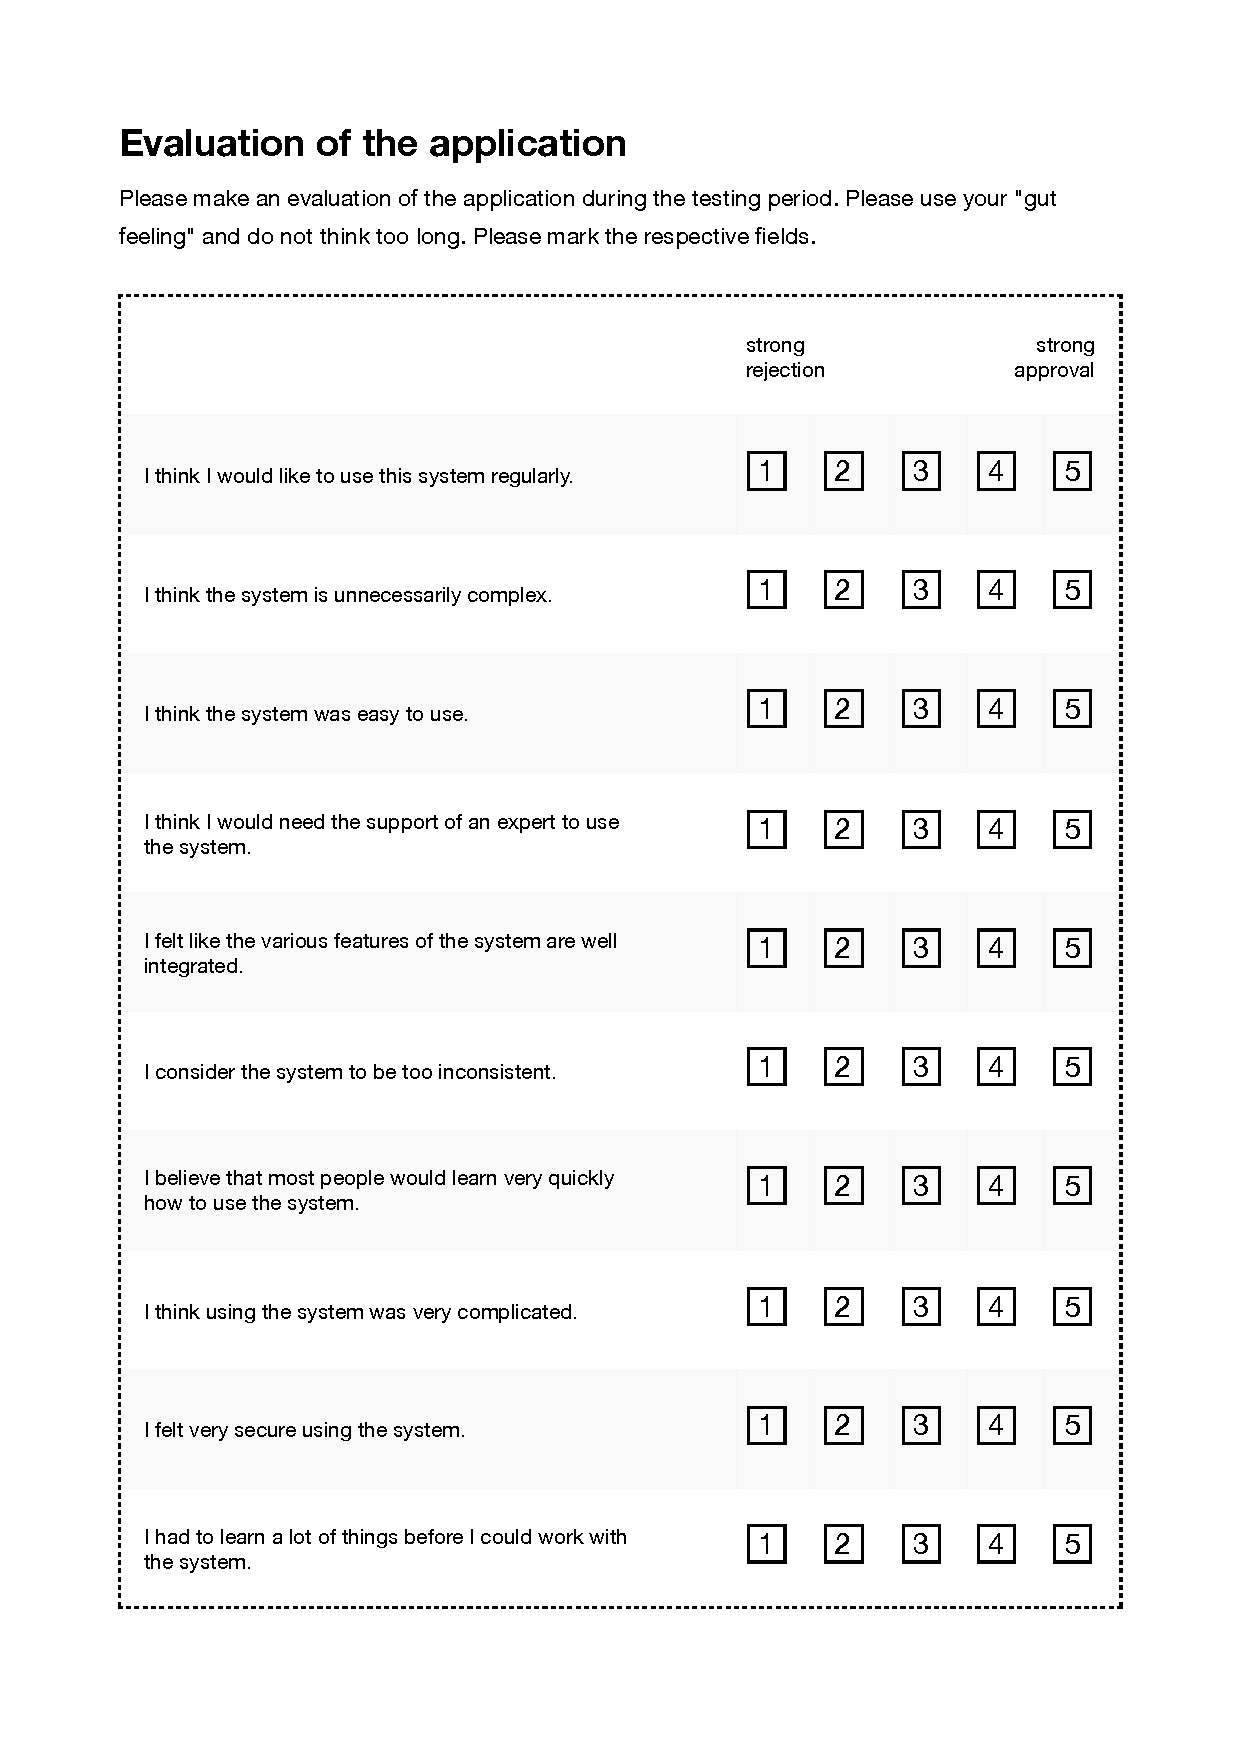
\includegraphics[width=.98\textwidth, page=1]{inlinepdf/sus}}}
\label{sus}
\vfill

\newpage
\section{Questionaire}
\vfill
\center{\frame{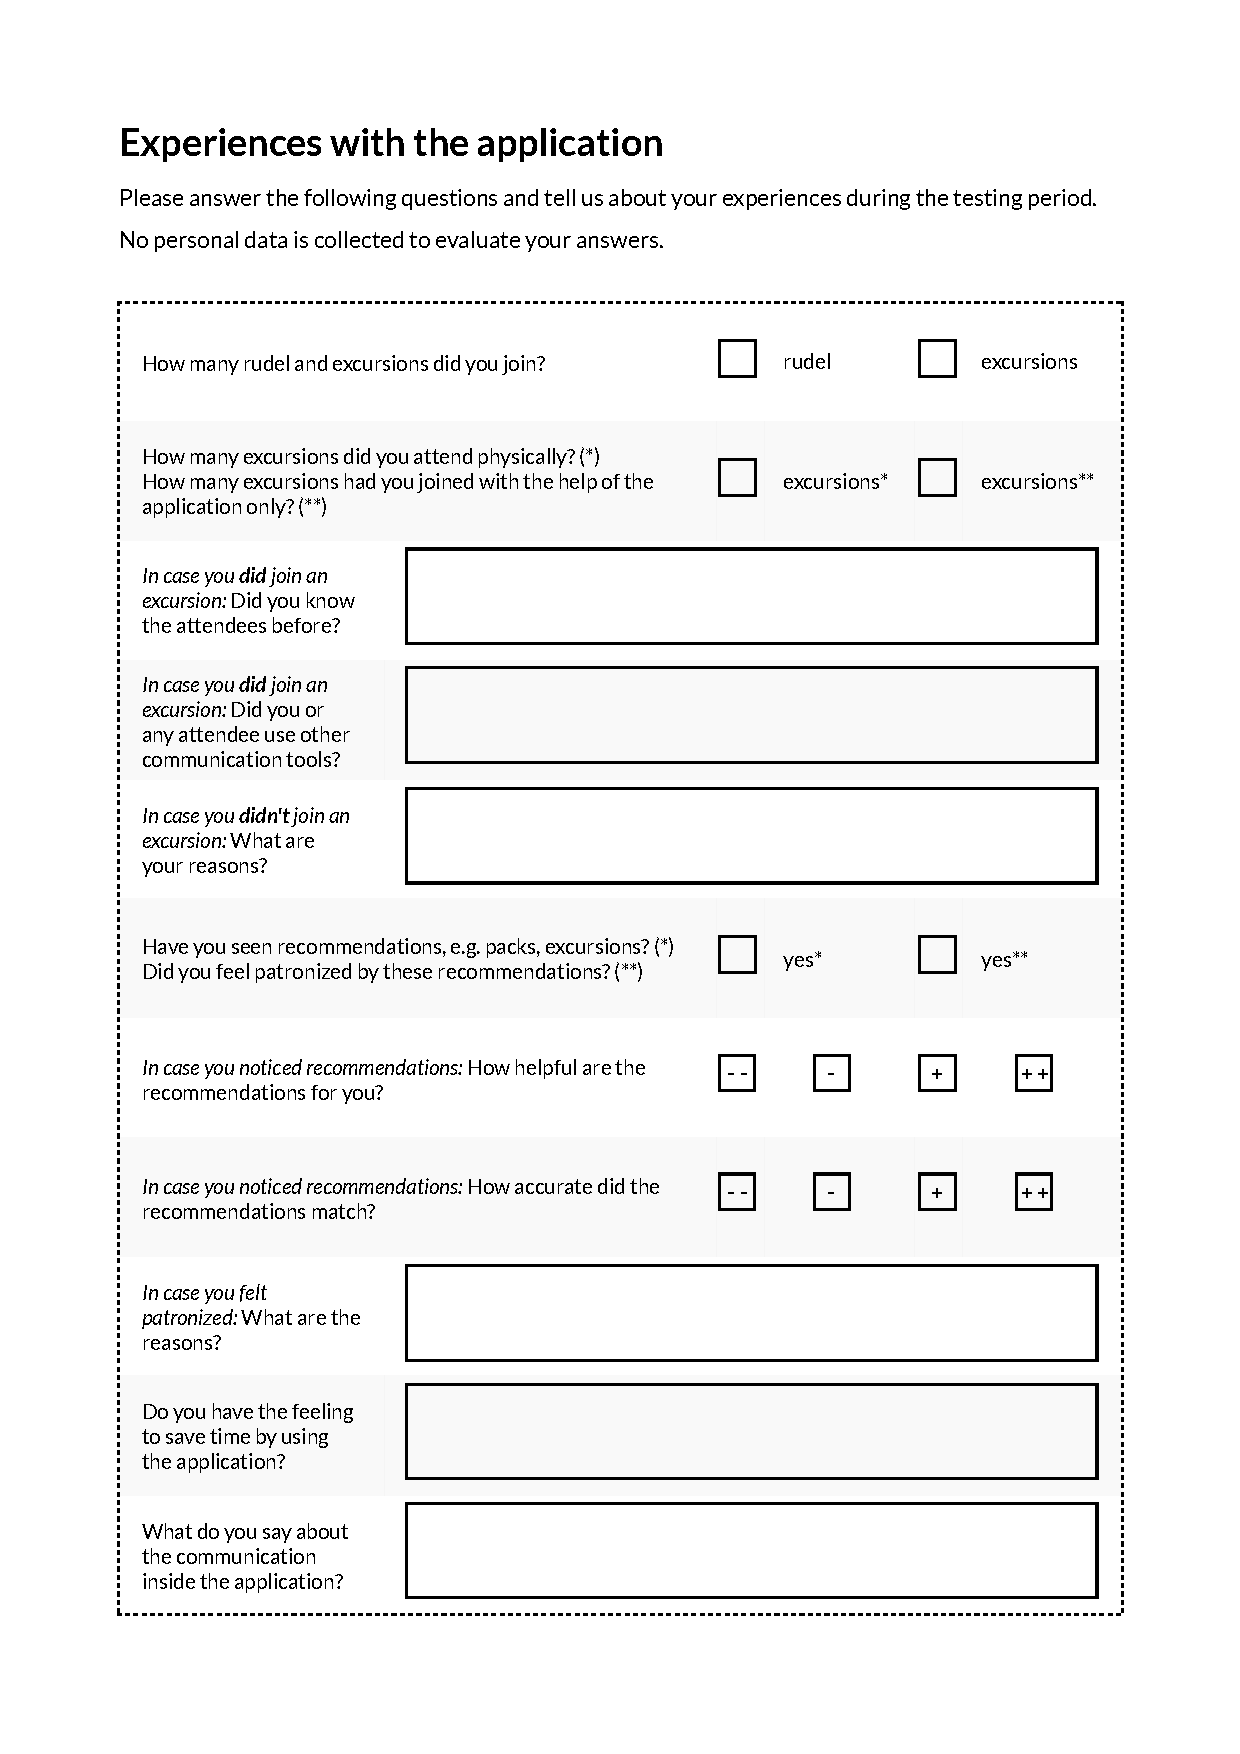
\includegraphics[width=.98\textwidth, page=1]{inlinepdf/qualitativequestionaire}}}
\label{qualitativequestionaire0}
\vfill
\clearpage
\vfill
\center{\frame{\includegraphics[width=.98\textwidth, page=2]{inlinepdf/qualitativequestionaire}}}
\label{qualitativequestionaire1}
\vfill
\clearpage
\vfill
\center{\frame{\includegraphics[width=.98\textwidth, page=3]{inlinepdf/qualitativequestionaire}}}
\label{qualitativequestionaire2}

% Literaturverzeichnis
\clearpage
\pagenumbering{roman}
\bibliographystyle{apalike}
\bibliography{books}

%Abbildungsverzeichnis
\listoffigures

% Erklärung
\chapter*{Declaration of academic honesty}
\thispagestyle{empty}
XXXX
\begin{center}
\begin{tabular}{lp{2em}l} 
 \hspace{5cm}   && \hspace{4cm} \\\cline{1-1}\cline{3-3} 
 Bremen, \today    && Jan-Hendrik Wolf 
\end{tabular} 
\end{center}
\end{document}